%! TEX encoding = utf8
\chapter{Laboratorium}

%%%%%%%%%%%%%% Podpunkt 1
\section{Określenie wartości pomiaru temperatury w punkcie pracy}

W celu określenia wartości pomiaru temperatury w punkcie pracy, ustawiono moc wentylatorów  $W1 = W2 = 50\%$ oraz moc grzałek $G1 = 25\%$  $G2 = 30\%$.
Po pewnym czasie temperatury, odczytywane przez czujniki zaczeły się stabilizować  na poziomie:  $T1 = 29,81^{\circ} C$ oraz $T3 = 31,43^{\circ} C$.


Niestety z powodu ciągłego ruchu powietrza związanego z przemieszczaniem się osób w sali i dużej ilości tych osób wpływających na temperaturę sali oraz czułość stanowiska pomiarowego temperatury odczytywane przez czujnik zaczeły lekko oscylować wokół temperatur w punkcie pracy.

\begin{figure}[H]
\centering
% This file was created by matlab2tikz.
%
%The latest updates can be retrieved from
%  http://www.mathworks.com/matlabcentral/fileexchange/22022-matlab2tikz-matlab2tikz
%where you can also make suggestions and rate matlab2tikz.
%
\definecolor{mycolor1}{rgb}{0.00000,0.44700,0.74100}%
%
\begin{tikzpicture}

\begin{axis}[%
width=4.658in,
height=3.209in,
at={(0.781in,0.433in)},
scale only axis,
xmin=0,
xmax=300,
ymin=0,
ymax=1,
axis background/.style={fill=white},
title style={font=\bfseries},
title={Sprawdzenie punktu pracy}
]
\addplot[const plot, color=mycolor1, forget plot] table[row sep=crcr] {%
1	0\\
2	0\\
3	0\\
4	0\\
5	0\\
6	0\\
7	0\\
8	0\\
9	0\\
10	0\\
11	0\\
12	0.0057600000000001\\
13	0.0163532160000003\\
14	0.0309651195456007\\
15	0.048881307228314\\
16	0.069476603547787\\
17	0.0922052763231956\\
18	0.116592255386335\\
19	0.142225255749747\\
20	0.168747715920214\\
21	0.195852470612454\\
22	0.223276084892824\\
23	0.250793783823562\\
24	0.278214918053031\\
25	0.305378911568507\\
26	0.332151643051804\\
27	0.3584222170054\\
28	0.384100085094331\\
29	0.409112482018918\\
30	0.433402143733736\\
31	0.456925278993718\\
32	0.479649768070473\\
33	0.501553565069219\\
34	0.522623282615215\\
35	0.542852939791618\\
36	0.5622428561196\\
37	0.580798676095743\\
38	0.59853051035856\\
39	0.615452180961476\\
40	0.631580559498089\\
41	0.646934987970007\\
42	0.661536773320006\\
43	0.675408747484182\\
44	0.688574885656094\\
45	0.701059976212247\\
46	0.712889336429715\\
47	0.724088568740435\\
48	0.73468335281921\\
49	0.744699269299771\\
50	0.754161651360567\\
51	0.763095460824262\\
52	0.771525185776541\\
53	0.779474757034723\\
54	0.786967481088494\\
55	0.794025987396991\\
56	0.800672188161484\\
57	0.80692724890363\\
58	0.812811568368131\\
59	0.81834476643781\\
60	0.823545678900522\\
61	0.828432358042782\\
62	0.833022078166089\\
63	0.837331345230081\\
64	0.841375909923215\\
65	0.845170783547751\\
66	0.84873025618259\\
67	0.852067916655778\\
68	0.855196673919261\\
69	0.858128779472453\\
70	0.860875850529054\\
71	0.863448893664023\\
72	0.86585832871519\\
73	0.868114012747174\\
74	0.870225263914635\\
75	0.87220088508767\\
76	0.874049187124909\\
77	0.875778011699796\\
78	0.877394753602984\\
79	0.87890638245907\\
80	0.880319463809153\\
81	0.88164017952227\\
82	0.882874347508767\\
83	0.884027440717295\\
84	0.885104605404514\\
85	0.886110678672969\\
86	0.887050205277941\\
87	0.887927453708666\\
88	0.888746431553108\\
89	0.889510900158644\\
90	0.89022438860361\\
91	0.890890206996765\\
92	0.891511459123398\\
93	0.892091054458077\\
94	0.892631719565016\\
95	0.893136008907717\\
96	0.893606315089962\\
97	0.894044878550474\\
98	0.894453796733613\\
99	0.894835032758363\\
100	0.895190423607635\\
101	0.895521687859606\\
102	0.895830432982346\\
103	0.896118162212535\\
104	0.8963862810385\\
105	0.896636103307207\\
106	0.896868856974233\\
107	0.897085689515068\\
108	0.897287673015447\\
109	0.897475808957719\\
110	0.897651032719581\\
111	0.89781421780083\\
112	0.8979661797931\\
113	0.898107680106889\\
114	0.898239429469513\\
115	0.898362091207007\\
116	0.898476284322334\\
117	0.898582586381679\\
118	0.898681536220013\\
119	0.898773636476516\\
120	0.89885935596994\\
121	0.898939131923422\\
122	0.899013372047781\\
123	0.899082456491821\\
124	0.899146739667709\\
125	0.899206551959049\\
126	0.89926220131884\\
127	0.899313974764102\\
128	0.89936213977358\\
129	0.899406945594544\\
130	0.899448624464363\\
131	0.899487392752224\\
132	0.899523452025996\\
133	0.899556990049003\\
134	0.899588181711143\\
135	0.89961718989853\\
136	0.899644166305616\\
137	0.899669252193451\\
138	0.899692579097577\\
139	0.899714269488791\\
140	0.899734437389834\\
141	0.899753188950872\\
142	0.899770622986443\\
143	0.899786831476406\\
144	0.89980190003322\\
145	0.899815908337794\\
146	0.899828930545949\\
147	0.89984103566745\\
148	0.899852287919408\\
149	0.899862747055753\\
150	0.899872468674377\\
151	0.899881504503407\\
152	0.899889902668031\\
153	0.899897707939144\\
154	0.899904961965061\\
155	0.899911703487396\\
156	0.899917968542212\\
157	0.899923790647388\\
158	0.899929200977171\\
159	0.899934228524749\\
160	0.899938900253668\\
161	0.899943241238845\\
162	0.899947274797884\\
163	0.899951022613345\\
164	0.899954504846591\\
165	0.899957740243783\\
166	0.899960746234549\\
167	0.89996353902384\\
168	0.899966133677433\\
169	0.899968544201511\\
170	0.899970783616728\\
171	0.899972864027148\\
172	0.899974796684384\\
173	0.899976592047297\\
174	0.899978259837537\\
175	0.899979809091224\\
176	0.899981248207034\\
177	0.899982584990925\\
178	0.899983826697764\\
179	0.89998498007003\\
180	0.899986051373833\\
181	0.899987046432406\\
182	0.899987970657262\\
183	0.899988829077171\\
184	0.89998962636511\\
185	0.899990366863326\\
186	0.899991054606642\\
187	0.899991693344134\\
188	0.89999228655928\\
189	0.899992837488707\\
190	0.89999334913961\\
191	0.899993824305955\\
192	0.899994265583541\\
193	0.899994675384006\\
194	0.899995055947841\\
195	0.899995409356498\\
196	0.899995737543635\\
197	0.899996042305581\\
198	0.89999632531105\\
199	0.899996588110183\\
200	0.899996832142945\\
201	0.899997058746931\\
202	0.89999726916462\\
203	0.899997464550123\\
204	0.899997645975445\\
205	0.899997814436311\\
206	0.899997970857582\\
207	0.899998116098277\\
208	0.899998250956257\\
209	0.899998376172558\\
210	0.899998492435436\\
211	0.899998600384113\\
212	0.899998700612261\\
213	0.899998793671242\\
214	0.899998880073114\\
215	0.899998960293429\\
216	0.899999034773827\\
217	0.899999103924452\\
218	0.899999168126188\\
219	0.899999227732749\\
220	0.899999283072606\\
221	0.899999334450791\\
222	0.899999382150561\\
223	0.899999426434952\\
224	0.899999467548222\\
225	0.899999505717183\\
226	0.89999954115245\\
227	0.899999574049592\\
228	0.899999604590208\\
229	0.899999632942922\\
230	0.899999659264306\\
231	0.899999683699746\\
232	0.899999706384231\\
233	0.899999727443105\\
234	0.899999746992746\\
235	0.899999765141214\\
236	0.899999781988841\\
237	0.89999979762878\\
238	0.899999812147525\\
239	0.899999825625379\\
240	0.899999838136903\\
241	0.89999984975132\\
242	0.899999860532901\\
243	0.899999870541317\\
244	0.899999879831968\\
245	0.89999988845629\\
246	0.899999896462033\\
247	0.899999903893532\\
248	0.899999910791946\\
249	0.899999917195486\\
250	0.899999923139629\\
251	0.899999928657308\\
252	0.899999933779098\\
253	0.899999938533386\\
254	0.899999942946523\\
255	0.899999947042972\\
256	0.899999950845445\\
257	0.899999954375025\\
258	0.899999957651284\\
259	0.899999960692394\\
260	0.89999996351522\\
261	0.899999966135423\\
262	0.899999968567538\\
263	0.899999970825058\\
264	0.899999972920511\\
265	0.899999974865526\\
266	0.899999976670896\\
267	0.899999978346643\\
268	0.899999979902069\\
269	0.899999981345808\\
270	0.899999982685876\\
271	0.899999983929714\\
272	0.899999985084229\\
273	0.899999986155833\\
274	0.899999987150476\\
275	0.899999988073684\\
276	0.899999988930584\\
277	0.899999989725938\\
278	0.899999990464164\\
279	0.899999991149363\\
280	0.899999991785343\\
281	0.899999992375638\\
282	0.899999992923528\\
283	0.899999993432058\\
284	0.899999993904056\\
285	0.899999994342144\\
286	0.899999994748757\\
287	0.899999995126157\\
288	0.899999995476441\\
289	0.899999995801557\\
290	0.899999996103313\\
291	0.899999996383386\\
292	0.899999996643334\\
293	0.899999996884603\\
294	0.899999997108535\\
295	0.899999997316374\\
296	0.899999997509277\\
297	0.899999997688318\\
298	0.899999997854491\\
299	0.899999998008722\\
300	0.899999998151869\\
};
\end{axis}
\end{tikzpicture}%
\caption{Pomiar temperatury w punkcie pracy}
\end{figure}

%%%%%%%%%%%%%% Podpunkt 2
\section{Mechanizm zabezpieczający przed uszkodzeniem stanowiska}

Zadaniem tego mechanizmu jest wyłączanie grzałki w moncie, gdy czujnik przy tej grzałce przekroczy temperaturę $250^{\circ} C$. 
W mechanizmie w tym uwzględniono również ograniczenia sygnału sterującego tzn. moc grzałki może przyjmować wartości z zakresu 0-100\% (w programie odpowiada to wartościom 0-1000). W programie wartości temperatur odpowiadają 100-krotnie większej wartości niż w rzeczywistości, dlatego też temperarura $250^{\circ} C$ zapisana jest jako 25000.

Implementacja przedstawia się w następujący sposób:



\begin{lstlisting}[style=customc,frame=single, caption=Mechanizm zabezpieczający , label=lst:overheat_lock] 
//mechanizm zabezpieczajacy
IF D100 >= 25000 THEN // T1>250  
	D114 := 0; //G1=0%
END_IF;

IF D102 >= 25000 THEN // T3>250 
	D115 := 0; //G2=0%
END_IF;

// zabezpieczenie sygnalu sterujacego
IF(D114>=1000) THEN //G1>100%
	D114 := 1000; //G1=100%
	ELSIF(D114<=0) THEN //G1<0%
	D114:=0; //G1=0%
END_IF;


IF(D115>=1000) THEN //G2>100%
	D115 := 1000; //G2=100%
	ELSIF(D115<=0) THEN //G2<0%
	D115:=0; //G2=0%
END_IF;
\end{lstlisting}


%%%%%%%%%%%%%% Podpunkt3
\section{Regulator PID}

W zadaniu tym użyto dwóch regulatorów PID (jeden ustala wartość sterowania grzałką G1, biorąc pod uwagę sygnał wyjściowy T1, natomiast drugi wyznacza G2, a bierze pod uwagę wartość T3). Dla każdego z regulatorów wartość sterowania jest liczona z wzoru: 
\begin{equation}
u(k)=r_2e(k-2) + r_1e(k-1) + r_0e(k) + u(k-1)
\label{control_rule}
\end{equation}
Współczynniki regulacji $r_i$ są wyliczane ze standardowych wzorów.
\begin{lstlisting}[style=customc,frame=single, caption=Wyznaczenie współczynników regulacji , label=lst:overheat_lock] 
//Wspolczynniki K, Ti i Td dla regulatorow
K_1 := 6.0;
K_2 := 6.0;

TI_1 := 100.0;
TI_2 := 110.0;

TD_1 := 0.0;
TD_2 := 0.0;

TProb := 4.0; //czas probkowania

//Wartosci uchybow w potrzednich chwilach probkowania
E0_1 := 0;
E1_1 := 0;
E2_1 := 0;
E0_2 := 0;
E1_2 := 0;
E2_2 := 0;


//wyliczenie wspolczynnikow ri dla PID1
R0_1 := K_1 * (1 + (TProb/(2*TI_1))+TD_1/TProb);
R1_1 := K_1 * (TProb/(2*TI_1) - 2*TD_1/TProb - 1);
R2_1 := K_1 * TD_1 / TProb;

//wyliczenie wspolczynnikow ri dla PID2
R0_2 := K_2 * (1 + (TProb/(2*TI_2))+TD_2/TProb);
R1_2 := K_2 * (TProb/(2*TI_2) - 2*TD_2/TProb - 1);
R2_2 := K_2 * TD_2 / TProb;
\end{lstlisting}

\begin{lstlisting}[style=customc,frame=single, caption=Implementacja algorytmu PID , label=lst:overheat_lock] 
T1_act := D100; //pobrane aktualnej wartosci T1
T3_act := D102; //pobrane aktualnej wartosci T3


// PID 1
E2_1 := E1_1; //przesuniecia wartosci uchybow w chwili k-2, k-1
E1_1 := E0_1;
E0_1 := y_zad1 - T1_act; //wyliczenie aktualnego uchybu

//wyliczenie nowego sterowania zgodnie ze wzorem
U_1 := R2_1*E2_1 + R1_1*E1_1 + R0_1*E0_1 + U_1; 
D114 := REAL_TO_INT(U_1); //zadanie nowej wartosci sterowania

// PID 2
E2_2 := E1_2;
E1_2 := E0_2;
E0_2 := y_zad2 - T3_act;

//wyliczenie nowego sterowania zgodnie ze wzorem
U_2 := R2_2*E2_2 + R1_2*E1_2 + R0_2*E0_2 + U_2; 
D115 := REAL_TO_INT(U_2); //zadanie nowej wartosci sterowania
\end{lstlisting}

Po każdym wyliczeniu nowej wartości sterowania, wykonywany jest mechanizm zabezpieczający z podpunktu drugiego.

\begin{figure}[H]
\centering
% This file was created by matlab2tikz.
%
%The latest updates can be retrieved from
%  http://www.mathworks.com/matlabcentral/fileexchange/22022-matlab2tikz-matlab2tikz
%where you can also make suggestions and rate matlab2tikz.
%
\definecolor{mycolor1}{rgb}{0.00000,0.44700,0.74100}%
\definecolor{mycolor2}{rgb}{0.85000,0.32500,0.09800}%
%
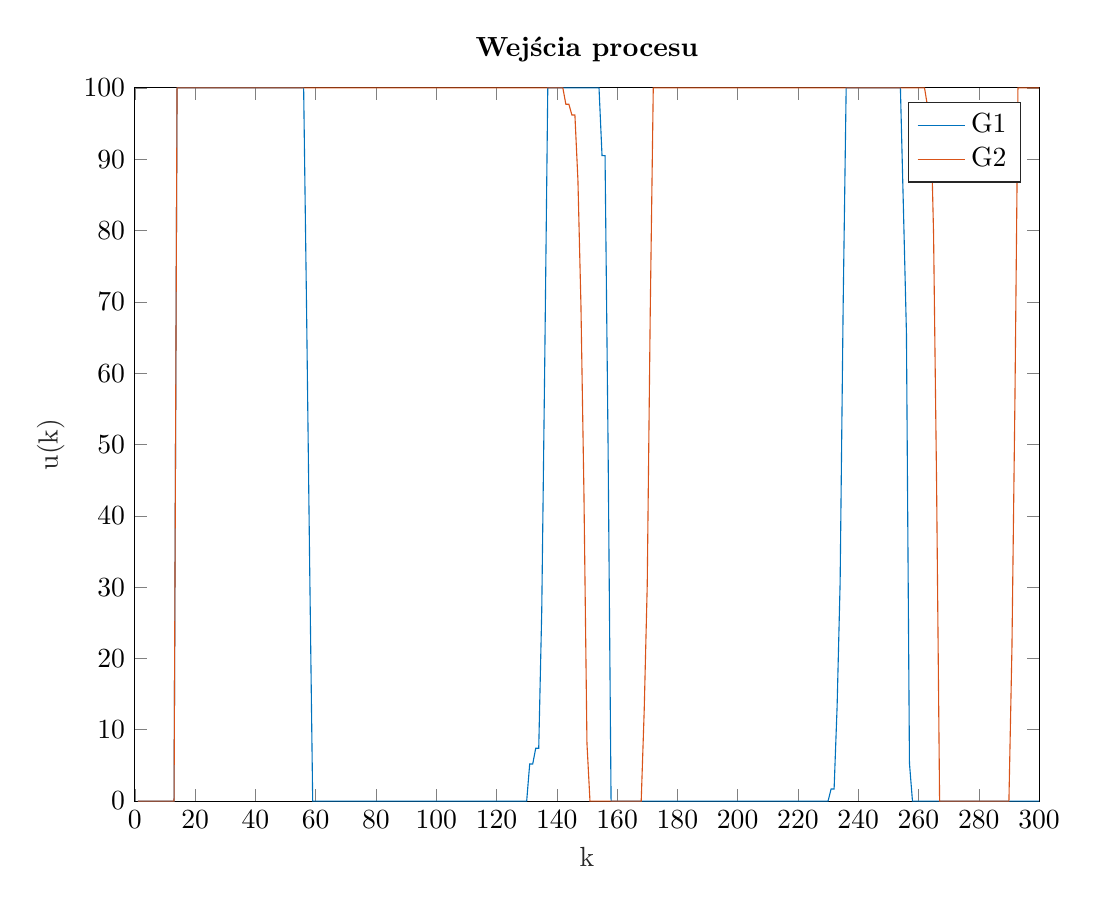
\begin{tikzpicture}

\begin{axis}[%
width=4.521in,
height=3.566in,
at={(0.758in,0.481in)},
scale only axis,
xmin=0,
xmax=300,
xlabel style={font=\color{white!15!black}},
xlabel={k},
ymin=0,
ymax=100,
ylabel style={font=\color{white!15!black}},
ylabel={u(k)},
axis background/.style={fill=white},
title style={font=\bfseries},
title={Wejścia procesu},
legend style={legend cell align=left, align=left, draw=white!15!black}
]
\addplot [color=mycolor1]
  table[row sep=crcr]{%
1	0\\
2	0\\
3	0\\
4	0\\
5	0\\
6	0\\
7	0\\
8	0\\
9	0\\
10	0\\
11	0\\
12	0\\
13	0\\
14	100\\
15	100\\
16	100\\
17	100\\
18	100\\
19	100\\
20	100\\
21	100\\
22	100\\
23	100\\
24	100\\
25	100\\
26	100\\
27	100\\
28	100\\
29	100\\
30	100\\
31	100\\
32	100\\
33	100\\
34	100\\
35	100\\
36	100\\
37	100\\
38	100\\
39	100\\
40	100\\
41	100\\
42	100\\
43	100\\
44	100\\
45	100\\
46	100\\
47	100\\
48	100\\
49	100\\
50	100\\
51	100\\
52	100\\
53	100\\
54	100\\
55	100\\
56	100\\
57	68\\
58	33\\
59	0\\
60	0\\
61	0\\
62	0\\
63	0\\
64	0\\
65	0\\
66	0\\
67	0\\
68	0\\
69	0\\
70	0\\
71	0\\
72	0\\
73	0\\
74	0\\
75	0\\
76	0\\
77	0\\
78	0\\
79	0\\
80	0\\
81	0\\
82	0\\
83	0\\
84	0\\
85	0\\
86	0\\
87	0\\
88	0\\
89	0\\
90	0\\
91	0\\
92	0\\
93	0\\
94	0\\
95	0\\
96	0\\
97	0\\
98	0\\
99	0\\
100	0\\
101	0\\
102	0\\
103	0\\
104	0\\
105	0\\
106	0\\
107	0\\
108	0\\
109	0\\
110	0\\
111	0\\
112	0\\
113	0\\
114	0\\
115	0\\
116	0\\
117	0\\
118	0\\
119	0\\
120	0\\
121	0\\
122	0\\
123	0\\
124	0\\
125	0\\
126	0\\
127	0\\
128	0\\
129	0\\
130	0\\
131	5.2\\
132	5.2\\
133	7.4\\
134	7.4\\
135	26.7\\
136	61.7\\
137	100\\
138	100\\
139	100\\
140	100\\
141	100\\
142	100\\
143	100\\
144	100\\
145	100\\
146	100\\
147	100\\
148	100\\
149	100\\
150	100\\
151	100\\
152	100\\
153	100\\
154	100\\
155	90.5\\
156	90.5\\
157	50.1\\
158	0\\
159	0\\
160	0\\
161	0\\
162	0\\
163	0\\
164	0\\
165	0\\
166	0\\
167	0\\
168	0\\
169	0\\
170	0\\
171	0\\
172	0\\
173	0\\
174	0\\
175	0\\
176	0\\
177	0\\
178	0\\
179	0\\
180	0\\
181	0\\
182	0\\
183	0\\
184	0\\
185	0\\
186	0\\
187	0\\
188	0\\
189	0\\
190	0\\
191	0\\
192	0\\
193	0\\
194	0\\
195	0\\
196	0\\
197	0\\
198	0\\
199	0\\
200	0\\
201	0\\
202	0\\
203	0\\
204	0\\
205	0\\
206	0\\
207	0\\
208	0\\
209	0\\
210	0\\
211	0\\
212	0\\
213	0\\
214	0\\
215	0\\
216	0\\
217	0\\
218	0\\
219	0\\
220	0\\
221	0\\
222	0\\
223	0\\
224	0\\
225	0\\
226	0\\
227	0\\
228	0\\
229	0\\
230	0\\
231	1.7\\
232	1.7\\
233	13.3\\
234	30.7\\
235	69.4\\
236	100\\
237	100\\
238	100\\
239	100\\
240	100\\
241	100\\
242	100\\
243	100\\
244	100\\
245	100\\
246	100\\
247	100\\
248	100\\
249	100\\
250	100\\
251	100\\
252	100\\
253	100\\
254	100\\
255	83.1\\
256	65.6\\
257	5.3\\
258	0\\
259	0\\
260	0\\
261	0\\
262	0\\
263	0\\
264	0\\
265	0\\
266	0\\
267	0\\
268	0\\
269	0\\
270	0\\
271	0\\
272	0\\
273	0\\
274	0\\
275	0\\
276	0\\
277	0\\
278	0\\
279	0\\
280	0\\
281	0\\
282	0\\
283	0\\
284	0\\
285	0\\
286	0\\
287	0\\
288	0\\
289	0\\
290	0\\
291	0\\
292	0\\
293	0\\
294	0\\
295	0\\
296	0\\
297	0\\
298	0\\
299	0\\
300	0\\
};
\addlegendentry{G1}

\addplot [color=mycolor2]
  table[row sep=crcr]{%
1	0\\
2	0\\
3	0\\
4	0\\
5	0\\
6	0\\
7	0\\
8	0\\
9	0\\
10	0\\
11	0\\
12	0\\
13	0\\
14	100\\
15	100\\
16	100\\
17	100\\
18	100\\
19	100\\
20	100\\
21	100\\
22	100\\
23	100\\
24	100\\
25	100\\
26	100\\
27	100\\
28	100\\
29	100\\
30	100\\
31	100\\
32	100\\
33	100\\
34	100\\
35	100\\
36	100\\
37	100\\
38	100\\
39	100\\
40	100\\
41	100\\
42	100\\
43	100\\
44	100\\
45	100\\
46	100\\
47	100\\
48	100\\
49	100\\
50	100\\
51	100\\
52	100\\
53	100\\
54	100\\
55	100\\
56	100\\
57	100\\
58	100\\
59	100\\
60	100\\
61	100\\
62	100\\
63	100\\
64	100\\
65	100\\
66	100\\
67	100\\
68	100\\
69	100\\
70	100\\
71	100\\
72	100\\
73	100\\
74	100\\
75	100\\
76	100\\
77	100\\
78	100\\
79	100\\
80	100\\
81	100\\
82	100\\
83	100\\
84	100\\
85	100\\
86	100\\
87	100\\
88	100\\
89	100\\
90	100\\
91	100\\
92	100\\
93	100\\
94	100\\
95	100\\
96	100\\
97	100\\
98	100\\
99	100\\
100	100\\
101	100\\
102	100\\
103	100\\
104	100\\
105	100\\
106	100\\
107	100\\
108	100\\
109	100\\
110	100\\
111	100\\
112	100\\
113	100\\
114	100\\
115	100\\
116	100\\
117	100\\
118	100\\
119	100\\
120	100\\
121	100\\
122	100\\
123	100\\
124	100\\
125	100\\
126	100\\
127	100\\
128	100\\
129	100\\
130	100\\
131	100\\
132	100\\
133	100\\
134	100\\
135	100\\
136	100\\
137	100\\
138	100\\
139	100\\
140	100\\
141	100\\
142	100\\
143	97.7\\
144	97.7\\
145	96.2\\
146	96.2\\
147	87.1\\
148	69.6\\
149	43.1\\
150	8.1\\
151	0\\
152	0\\
153	0\\
154	0\\
155	0\\
156	0\\
157	0\\
158	0\\
159	0\\
160	0\\
161	0\\
162	0\\
163	0\\
164	0\\
165	0\\
166	0\\
167	0\\
168	0\\
169	12.8\\
170	30.3\\
171	68.7\\
172	100\\
173	100\\
174	100\\
175	100\\
176	100\\
177	100\\
178	100\\
179	100\\
180	100\\
181	100\\
182	100\\
183	100\\
184	100\\
185	100\\
186	100\\
187	100\\
188	100\\
189	100\\
190	100\\
191	100\\
192	100\\
193	100\\
194	100\\
195	100\\
196	100\\
197	100\\
198	100\\
199	100\\
200	100\\
201	100\\
202	100\\
203	100\\
204	100\\
205	100\\
206	100\\
207	100\\
208	100\\
209	100\\
210	100\\
211	100\\
212	100\\
213	100\\
214	100\\
215	100\\
216	100\\
217	100\\
218	100\\
219	100\\
220	100\\
221	100\\
222	100\\
223	100\\
224	100\\
225	100\\
226	100\\
227	100\\
228	100\\
229	100\\
230	100\\
231	100\\
232	100\\
233	100\\
234	100\\
235	100\\
236	100\\
237	100\\
238	100\\
239	100\\
240	100\\
241	100\\
242	100\\
243	100\\
244	100\\
245	100\\
246	100\\
247	100\\
248	100\\
249	100\\
250	100\\
251	100\\
252	100\\
253	100\\
254	100\\
255	100\\
256	100\\
257	100\\
258	100\\
259	100\\
260	100\\
261	100\\
262	100\\
263	97.4\\
264	97.4\\
265	79.5\\
266	44.5\\
267	0\\
268	0\\
269	0\\
270	0\\
271	0\\
272	0\\
273	0\\
274	0\\
275	0\\
276	0\\
277	0\\
278	0\\
279	0\\
280	0\\
281	0\\
282	0\\
283	0\\
284	0\\
285	0\\
286	0\\
287	0\\
288	0\\
289	0\\
290	0\\
291	21.4\\
292	56.4\\
293	100\\
294	100\\
295	100\\
296	100\\
297	100\\
298	100\\
299	100\\
300	100\\
};
\addlegendentry{G2}

\end{axis}
\end{tikzpicture}%
\caption{Sygnały stejące: PID1: K=3 $T_i$=100 $T_d$=1.3 PID2: K=2 $T_i$=90 $T_d$=1}
\end{figure}

\begin{figure}[H]
\centering
% This file was created by matlab2tikz.
%
%The latest updates can be retrieved from
%  http://www.mathworks.com/matlabcentral/fileexchange/22022-matlab2tikz-matlab2tikz
%where you can also make suggestions and rate matlab2tikz.
%
\definecolor{mycolor1}{rgb}{0.00000,0.44700,0.74100}%
\definecolor{mycolor2}{rgb}{0.85000,0.32500,0.09800}%
\definecolor{mycolor3}{rgb}{0.92900,0.69400,0.12500}%
\definecolor{mycolor4}{rgb}{0.49400,0.18400,0.55600}%
%
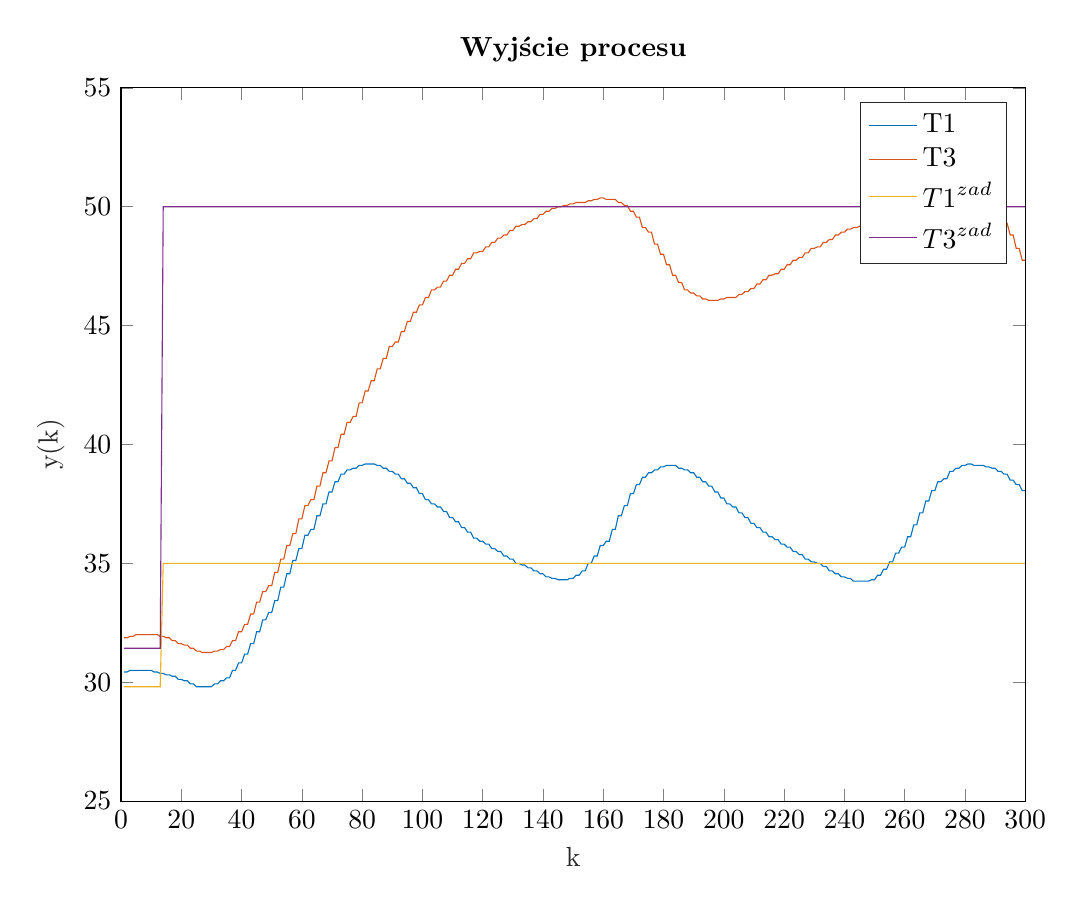
\begin{tikzpicture}

\begin{axis}[%
width=4.521in,
height=3.566in,
at={(0.758in,0.481in)},
scale only axis,
xmin=0,
xmax=300,
xlabel style={font=\color{white!15!black}},
xlabel={k},
ymin=25,
ymax=55,
ylabel style={font=\color{white!15!black}},
ylabel={y(k)},
axis background/.style={fill=white},
title style={font=\bfseries},
title={Wyjście procesu},
legend style={legend cell align=left, align=left, draw=white!15!black}
]
\addplot [color=mycolor1]
  table[row sep=crcr]{%
1	30.43\\
2	30.43\\
3	30.5\\
4	30.5\\
5	30.5\\
6	30.5\\
7	30.5\\
8	30.5\\
9	30.5\\
10	30.5\\
11	30.43\\
12	30.43\\
13	30.37\\
14	30.37\\
15	30.31\\
16	30.31\\
17	30.25\\
18	30.25\\
19	30.12\\
20	30.12\\
21	30.06\\
22	30.06\\
23	29.93\\
24	29.93\\
25	29.81\\
26	29.81\\
27	29.81\\
28	29.81\\
29	29.81\\
30	29.81\\
31	29.93\\
32	29.93\\
33	30.06\\
34	30.06\\
35	30.18\\
36	30.18\\
37	30.5\\
38	30.5\\
39	30.81\\
40	30.81\\
41	31.18\\
42	31.18\\
43	31.62\\
44	31.62\\
45	32.12\\
46	32.12\\
47	32.62\\
48	32.62\\
49	32.93\\
50	32.93\\
51	33.43\\
52	33.43\\
53	34\\
54	34\\
55	34.56\\
56	34.56\\
57	35.12\\
58	35.12\\
59	35.62\\
60	35.62\\
61	36.18\\
62	36.18\\
63	36.43\\
64	36.43\\
65	37\\
66	37\\
67	37.5\\
68	37.5\\
69	38\\
70	38\\
71	38.43\\
72	38.43\\
73	38.75\\
74	38.75\\
75	38.93\\
76	38.93\\
77	39\\
78	39\\
79	39.12\\
80	39.12\\
81	39.18\\
82	39.18\\
83	39.18\\
84	39.18\\
85	39.12\\
86	39.12\\
87	39\\
88	39\\
89	38.87\\
90	38.87\\
91	38.75\\
92	38.75\\
93	38.56\\
94	38.56\\
95	38.37\\
96	38.37\\
97	38.18\\
98	38.18\\
99	37.93\\
100	37.93\\
101	37.68\\
102	37.68\\
103	37.5\\
104	37.5\\
105	37.37\\
106	37.37\\
107	37.18\\
108	37.18\\
109	36.93\\
110	36.93\\
111	36.75\\
112	36.75\\
113	36.5\\
114	36.5\\
115	36.31\\
116	36.31\\
117	36.06\\
118	36.06\\
119	35.93\\
120	35.93\\
121	35.81\\
122	35.81\\
123	35.62\\
124	35.62\\
125	35.5\\
126	35.5\\
127	35.31\\
128	35.31\\
129	35.18\\
130	35.18\\
131	35\\
132	35\\
133	34.93\\
134	34.93\\
135	34.81\\
136	34.81\\
137	34.68\\
138	34.68\\
139	34.56\\
140	34.56\\
141	34.43\\
142	34.43\\
143	34.37\\
144	34.37\\
145	34.31\\
146	34.31\\
147	34.31\\
148	34.31\\
149	34.37\\
150	34.37\\
151	34.5\\
152	34.5\\
153	34.68\\
154	34.68\\
155	35\\
156	35\\
157	35.31\\
158	35.31\\
159	35.75\\
160	35.75\\
161	35.93\\
162	35.93\\
163	36.43\\
164	36.43\\
165	37\\
166	37\\
167	37.43\\
168	37.43\\
169	37.93\\
170	37.93\\
171	38.31\\
172	38.31\\
173	38.62\\
174	38.62\\
175	38.81\\
176	38.81\\
177	38.93\\
178	38.93\\
179	39.06\\
180	39.06\\
181	39.12\\
182	39.12\\
183	39.12\\
184	39.12\\
185	39\\
186	39\\
187	38.93\\
188	38.93\\
189	38.81\\
190	38.81\\
191	38.62\\
192	38.62\\
193	38.43\\
194	38.43\\
195	38.25\\
196	38.25\\
197	38\\
198	38\\
199	37.75\\
200	37.75\\
201	37.5\\
202	37.5\\
203	37.37\\
204	37.37\\
205	37.12\\
206	37.12\\
207	36.93\\
208	36.93\\
209	36.68\\
210	36.68\\
211	36.5\\
212	36.5\\
213	36.31\\
214	36.31\\
215	36.12\\
216	36.12\\
217	36\\
218	36\\
219	35.81\\
220	35.81\\
221	35.68\\
222	35.68\\
223	35.5\\
224	35.5\\
225	35.37\\
226	35.37\\
227	35.18\\
228	35.18\\
229	35.06\\
230	35.06\\
231	35\\
232	35\\
233	34.87\\
234	34.87\\
235	34.68\\
236	34.68\\
237	34.56\\
238	34.56\\
239	34.43\\
240	34.43\\
241	34.37\\
242	34.37\\
243	34.25\\
244	34.25\\
245	34.25\\
246	34.25\\
247	34.25\\
248	34.25\\
249	34.31\\
250	34.31\\
251	34.5\\
252	34.5\\
253	34.75\\
254	34.75\\
255	35.06\\
256	35.06\\
257	35.43\\
258	35.43\\
259	35.68\\
260	35.68\\
261	36.12\\
262	36.12\\
263	36.62\\
264	36.62\\
265	37.12\\
266	37.12\\
267	37.62\\
268	37.62\\
269	38.06\\
270	38.06\\
271	38.43\\
272	38.43\\
273	38.56\\
274	38.56\\
275	38.87\\
276	38.87\\
277	39\\
278	39\\
279	39.12\\
280	39.12\\
281	39.18\\
282	39.18\\
283	39.12\\
284	39.12\\
285	39.12\\
286	39.12\\
287	39.06\\
288	39.06\\
289	39\\
290	39\\
291	38.87\\
292	38.87\\
293	38.75\\
294	38.75\\
295	38.5\\
296	38.5\\
297	38.31\\
298	38.31\\
299	38.06\\
300	38.06\\
};
\addlegendentry{T1}

\addplot [color=mycolor2]
  table[row sep=crcr]{%
1	31.87\\
2	31.87\\
3	31.93\\
4	31.93\\
5	32\\
6	32\\
7	32\\
8	32\\
9	32\\
10	32\\
11	32\\
12	32\\
13	31.93\\
14	31.93\\
15	31.87\\
16	31.87\\
17	31.75\\
18	31.75\\
19	31.62\\
20	31.62\\
21	31.56\\
22	31.56\\
23	31.43\\
24	31.43\\
25	31.31\\
26	31.31\\
27	31.25\\
28	31.25\\
29	31.25\\
30	31.25\\
31	31.31\\
32	31.31\\
33	31.37\\
34	31.37\\
35	31.5\\
36	31.5\\
37	31.75\\
38	31.75\\
39	32.12\\
40	32.12\\
41	32.43\\
42	32.43\\
43	32.87\\
44	32.87\\
45	33.37\\
46	33.37\\
47	33.81\\
48	33.81\\
49	34.06\\
50	34.06\\
51	34.62\\
52	34.62\\
53	35.18\\
54	35.18\\
55	35.75\\
56	35.75\\
57	36.25\\
58	36.25\\
59	36.87\\
60	36.87\\
61	37.43\\
62	37.43\\
63	37.68\\
64	37.68\\
65	38.25\\
66	38.25\\
67	38.81\\
68	38.81\\
69	39.31\\
70	39.31\\
71	39.87\\
72	39.87\\
73	40.43\\
74	40.43\\
75	40.93\\
76	40.93\\
77	41.18\\
78	41.18\\
79	41.75\\
80	41.75\\
81	42.25\\
82	42.25\\
83	42.68\\
84	42.68\\
85	43.18\\
86	43.18\\
87	43.62\\
88	43.62\\
89	44.12\\
90	44.12\\
91	44.31\\
92	44.31\\
93	44.75\\
94	44.75\\
95	45.18\\
96	45.18\\
97	45.56\\
98	45.56\\
99	45.87\\
100	45.87\\
101	46.18\\
102	46.18\\
103	46.5\\
104	46.5\\
105	46.62\\
106	46.62\\
107	46.87\\
108	46.87\\
109	47.12\\
110	47.12\\
111	47.37\\
112	47.37\\
113	47.62\\
114	47.62\\
115	47.81\\
116	47.81\\
117	48.06\\
118	48.06\\
119	48.12\\
120	48.12\\
121	48.31\\
122	48.31\\
123	48.5\\
124	48.5\\
125	48.68\\
126	48.68\\
127	48.81\\
128	48.81\\
129	49\\
130	49\\
131	49.18\\
132	49.18\\
133	49.25\\
134	49.25\\
135	49.37\\
136	49.37\\
137	49.5\\
138	49.5\\
139	49.68\\
140	49.68\\
141	49.81\\
142	49.81\\
143	49.93\\
144	49.93\\
145	50\\
146	50\\
147	50.06\\
148	50.06\\
149	50.12\\
150	50.12\\
151	50.18\\
152	50.18\\
153	50.18\\
154	50.18\\
155	50.25\\
156	50.25\\
157	50.31\\
158	50.31\\
159	50.37\\
160	50.37\\
161	50.31\\
162	50.31\\
163	50.31\\
164	50.31\\
165	50.18\\
166	50.18\\
167	50.06\\
168	50.06\\
169	49.81\\
170	49.81\\
171	49.56\\
172	49.56\\
173	49.12\\
174	49.12\\
175	48.93\\
176	48.93\\
177	48.43\\
178	48.43\\
179	48\\
180	48\\
181	47.56\\
182	47.56\\
183	47.12\\
184	47.12\\
185	46.81\\
186	46.81\\
187	46.5\\
188	46.5\\
189	46.37\\
190	46.37\\
191	46.25\\
192	46.25\\
193	46.12\\
194	46.12\\
195	46.06\\
196	46.06\\
197	46.06\\
198	46.06\\
199	46.12\\
200	46.12\\
201	46.18\\
202	46.18\\
203	46.18\\
204	46.18\\
205	46.31\\
206	46.31\\
207	46.43\\
208	46.43\\
209	46.56\\
210	46.56\\
211	46.75\\
212	46.75\\
213	46.93\\
214	46.93\\
215	47.12\\
216	47.12\\
217	47.18\\
218	47.18\\
219	47.37\\
220	47.37\\
221	47.56\\
222	47.56\\
223	47.75\\
224	47.75\\
225	47.87\\
226	47.87\\
227	48.06\\
228	48.06\\
229	48.25\\
230	48.25\\
231	48.31\\
232	48.31\\
233	48.5\\
234	48.5\\
235	48.62\\
236	48.62\\
237	48.81\\
238	48.81\\
239	48.93\\
240	48.93\\
241	49.06\\
242	49.06\\
243	49.12\\
244	49.12\\
245	49.18\\
246	49.18\\
247	49.31\\
248	49.31\\
249	49.43\\
250	49.43\\
251	49.5\\
252	49.5\\
253	49.62\\
254	49.62\\
255	49.75\\
256	49.75\\
257	49.81\\
258	49.81\\
259	49.81\\
260	49.81\\
261	49.87\\
262	49.87\\
263	50\\
264	50\\
265	50.12\\
266	50.12\\
267	50.31\\
268	50.31\\
269	50.43\\
270	50.43\\
271	50.5\\
272	50.5\\
273	50.62\\
274	50.62\\
275	50.75\\
276	50.75\\
277	50.81\\
278	50.81\\
279	50.87\\
280	50.87\\
281	50.81\\
282	50.81\\
283	50.68\\
284	50.68\\
285	50.5\\
286	50.5\\
287	50.37\\
288	50.37\\
289	50.06\\
290	50.06\\
291	49.75\\
292	49.75\\
293	49.31\\
294	49.31\\
295	48.81\\
296	48.81\\
297	48.25\\
298	48.25\\
299	47.75\\
300	47.75\\
};
\addlegendentry{T3}

\addplot [color=mycolor3]
  table[row sep=crcr]{%
1	29.81\\
2	29.81\\
3	29.81\\
4	29.81\\
5	29.81\\
6	29.81\\
7	29.81\\
8	29.81\\
9	29.81\\
10	29.81\\
11	29.81\\
12	29.81\\
13	29.81\\
14	35\\
15	35\\
16	35\\
17	35\\
18	35\\
19	35\\
20	35\\
21	35\\
22	35\\
23	35\\
24	35\\
25	35\\
26	35\\
27	35\\
28	35\\
29	35\\
30	35\\
31	35\\
32	35\\
33	35\\
34	35\\
35	35\\
36	35\\
37	35\\
38	35\\
39	35\\
40	35\\
41	35\\
42	35\\
43	35\\
44	35\\
45	35\\
46	35\\
47	35\\
48	35\\
49	35\\
50	35\\
51	35\\
52	35\\
53	35\\
54	35\\
55	35\\
56	35\\
57	35\\
58	35\\
59	35\\
60	35\\
61	35\\
62	35\\
63	35\\
64	35\\
65	35\\
66	35\\
67	35\\
68	35\\
69	35\\
70	35\\
71	35\\
72	35\\
73	35\\
74	35\\
75	35\\
76	35\\
77	35\\
78	35\\
79	35\\
80	35\\
81	35\\
82	35\\
83	35\\
84	35\\
85	35\\
86	35\\
87	35\\
88	35\\
89	35\\
90	35\\
91	35\\
92	35\\
93	35\\
94	35\\
95	35\\
96	35\\
97	35\\
98	35\\
99	35\\
100	35\\
101	35\\
102	35\\
103	35\\
104	35\\
105	35\\
106	35\\
107	35\\
108	35\\
109	35\\
110	35\\
111	35\\
112	35\\
113	35\\
114	35\\
115	35\\
116	35\\
117	35\\
118	35\\
119	35\\
120	35\\
121	35\\
122	35\\
123	35\\
124	35\\
125	35\\
126	35\\
127	35\\
128	35\\
129	35\\
130	35\\
131	35\\
132	35\\
133	35\\
134	35\\
135	35\\
136	35\\
137	35\\
138	35\\
139	35\\
140	35\\
141	35\\
142	35\\
143	35\\
144	35\\
145	35\\
146	35\\
147	35\\
148	35\\
149	35\\
150	35\\
151	35\\
152	35\\
153	35\\
154	35\\
155	35\\
156	35\\
157	35\\
158	35\\
159	35\\
160	35\\
161	35\\
162	35\\
163	35\\
164	35\\
165	35\\
166	35\\
167	35\\
168	35\\
169	35\\
170	35\\
171	35\\
172	35\\
173	35\\
174	35\\
175	35\\
176	35\\
177	35\\
178	35\\
179	35\\
180	35\\
181	35\\
182	35\\
183	35\\
184	35\\
185	35\\
186	35\\
187	35\\
188	35\\
189	35\\
190	35\\
191	35\\
192	35\\
193	35\\
194	35\\
195	35\\
196	35\\
197	35\\
198	35\\
199	35\\
200	35\\
201	35\\
202	35\\
203	35\\
204	35\\
205	35\\
206	35\\
207	35\\
208	35\\
209	35\\
210	35\\
211	35\\
212	35\\
213	35\\
214	35\\
215	35\\
216	35\\
217	35\\
218	35\\
219	35\\
220	35\\
221	35\\
222	35\\
223	35\\
224	35\\
225	35\\
226	35\\
227	35\\
228	35\\
229	35\\
230	35\\
231	35\\
232	35\\
233	35\\
234	35\\
235	35\\
236	35\\
237	35\\
238	35\\
239	35\\
240	35\\
241	35\\
242	35\\
243	35\\
244	35\\
245	35\\
246	35\\
247	35\\
248	35\\
249	35\\
250	35\\
251	35\\
252	35\\
253	35\\
254	35\\
255	35\\
256	35\\
257	35\\
258	35\\
259	35\\
260	35\\
261	35\\
262	35\\
263	35\\
264	35\\
265	35\\
266	35\\
267	35\\
268	35\\
269	35\\
270	35\\
271	35\\
272	35\\
273	35\\
274	35\\
275	35\\
276	35\\
277	35\\
278	35\\
279	35\\
280	35\\
281	35\\
282	35\\
283	35\\
284	35\\
285	35\\
286	35\\
287	35\\
288	35\\
289	35\\
290	35\\
291	35\\
292	35\\
293	35\\
294	35\\
295	35\\
296	35\\
297	35\\
298	35\\
299	35\\
300	35\\
};
\addlegendentry{$\text{T1}^{\text{zad}}$}

\addplot [color=mycolor4]
  table[row sep=crcr]{%
1	31.43\\
2	31.43\\
3	31.43\\
4	31.43\\
5	31.43\\
6	31.43\\
7	31.43\\
8	31.43\\
9	31.43\\
10	31.43\\
11	31.43\\
12	31.43\\
13	31.43\\
14	50\\
15	50\\
16	50\\
17	50\\
18	50\\
19	50\\
20	50\\
21	50\\
22	50\\
23	50\\
24	50\\
25	50\\
26	50\\
27	50\\
28	50\\
29	50\\
30	50\\
31	50\\
32	50\\
33	50\\
34	50\\
35	50\\
36	50\\
37	50\\
38	50\\
39	50\\
40	50\\
41	50\\
42	50\\
43	50\\
44	50\\
45	50\\
46	50\\
47	50\\
48	50\\
49	50\\
50	50\\
51	50\\
52	50\\
53	50\\
54	50\\
55	50\\
56	50\\
57	50\\
58	50\\
59	50\\
60	50\\
61	50\\
62	50\\
63	50\\
64	50\\
65	50\\
66	50\\
67	50\\
68	50\\
69	50\\
70	50\\
71	50\\
72	50\\
73	50\\
74	50\\
75	50\\
76	50\\
77	50\\
78	50\\
79	50\\
80	50\\
81	50\\
82	50\\
83	50\\
84	50\\
85	50\\
86	50\\
87	50\\
88	50\\
89	50\\
90	50\\
91	50\\
92	50\\
93	50\\
94	50\\
95	50\\
96	50\\
97	50\\
98	50\\
99	50\\
100	50\\
101	50\\
102	50\\
103	50\\
104	50\\
105	50\\
106	50\\
107	50\\
108	50\\
109	50\\
110	50\\
111	50\\
112	50\\
113	50\\
114	50\\
115	50\\
116	50\\
117	50\\
118	50\\
119	50\\
120	50\\
121	50\\
122	50\\
123	50\\
124	50\\
125	50\\
126	50\\
127	50\\
128	50\\
129	50\\
130	50\\
131	50\\
132	50\\
133	50\\
134	50\\
135	50\\
136	50\\
137	50\\
138	50\\
139	50\\
140	50\\
141	50\\
142	50\\
143	50\\
144	50\\
145	50\\
146	50\\
147	50\\
148	50\\
149	50\\
150	50\\
151	50\\
152	50\\
153	50\\
154	50\\
155	50\\
156	50\\
157	50\\
158	50\\
159	50\\
160	50\\
161	50\\
162	50\\
163	50\\
164	50\\
165	50\\
166	50\\
167	50\\
168	50\\
169	50\\
170	50\\
171	50\\
172	50\\
173	50\\
174	50\\
175	50\\
176	50\\
177	50\\
178	50\\
179	50\\
180	50\\
181	50\\
182	50\\
183	50\\
184	50\\
185	50\\
186	50\\
187	50\\
188	50\\
189	50\\
190	50\\
191	50\\
192	50\\
193	50\\
194	50\\
195	50\\
196	50\\
197	50\\
198	50\\
199	50\\
200	50\\
201	50\\
202	50\\
203	50\\
204	50\\
205	50\\
206	50\\
207	50\\
208	50\\
209	50\\
210	50\\
211	50\\
212	50\\
213	50\\
214	50\\
215	50\\
216	50\\
217	50\\
218	50\\
219	50\\
220	50\\
221	50\\
222	50\\
223	50\\
224	50\\
225	50\\
226	50\\
227	50\\
228	50\\
229	50\\
230	50\\
231	50\\
232	50\\
233	50\\
234	50\\
235	50\\
236	50\\
237	50\\
238	50\\
239	50\\
240	50\\
241	50\\
242	50\\
243	50\\
244	50\\
245	50\\
246	50\\
247	50\\
248	50\\
249	50\\
250	50\\
251	50\\
252	50\\
253	50\\
254	50\\
255	50\\
256	50\\
257	50\\
258	50\\
259	50\\
260	50\\
261	50\\
262	50\\
263	50\\
264	50\\
265	50\\
266	50\\
267	50\\
268	50\\
269	50\\
270	50\\
271	50\\
272	50\\
273	50\\
274	50\\
275	50\\
276	50\\
277	50\\
278	50\\
279	50\\
280	50\\
281	50\\
282	50\\
283	50\\
284	50\\
285	50\\
286	50\\
287	50\\
288	50\\
289	50\\
290	50\\
291	50\\
292	50\\
293	50\\
294	50\\
295	50\\
296	50\\
297	50\\
298	50\\
299	50\\
300	50\\
};
\addlegendentry{$\text{T3}^{\text{zad}}$}

\end{axis}
\end{tikzpicture}%
\caption{Wyjścia obiektu: PID1: K=3 $T_i$=100 $T_d$=1.3 PID2: K=2 $T_i$=90 $T_d$=1}
\end{figure}

\begin{figure}[H]
\centering
% This file was created by matlab2tikz.
%
%The latest updates can be retrieved from
%  http://www.mathworks.com/matlabcentral/fileexchange/22022-matlab2tikz-matlab2tikz
%where you can also make suggestions and rate matlab2tikz.
%
\definecolor{mycolor1}{rgb}{0.00000,0.44700,0.74100}%
\definecolor{mycolor2}{rgb}{0.85000,0.32500,0.09800}%
%
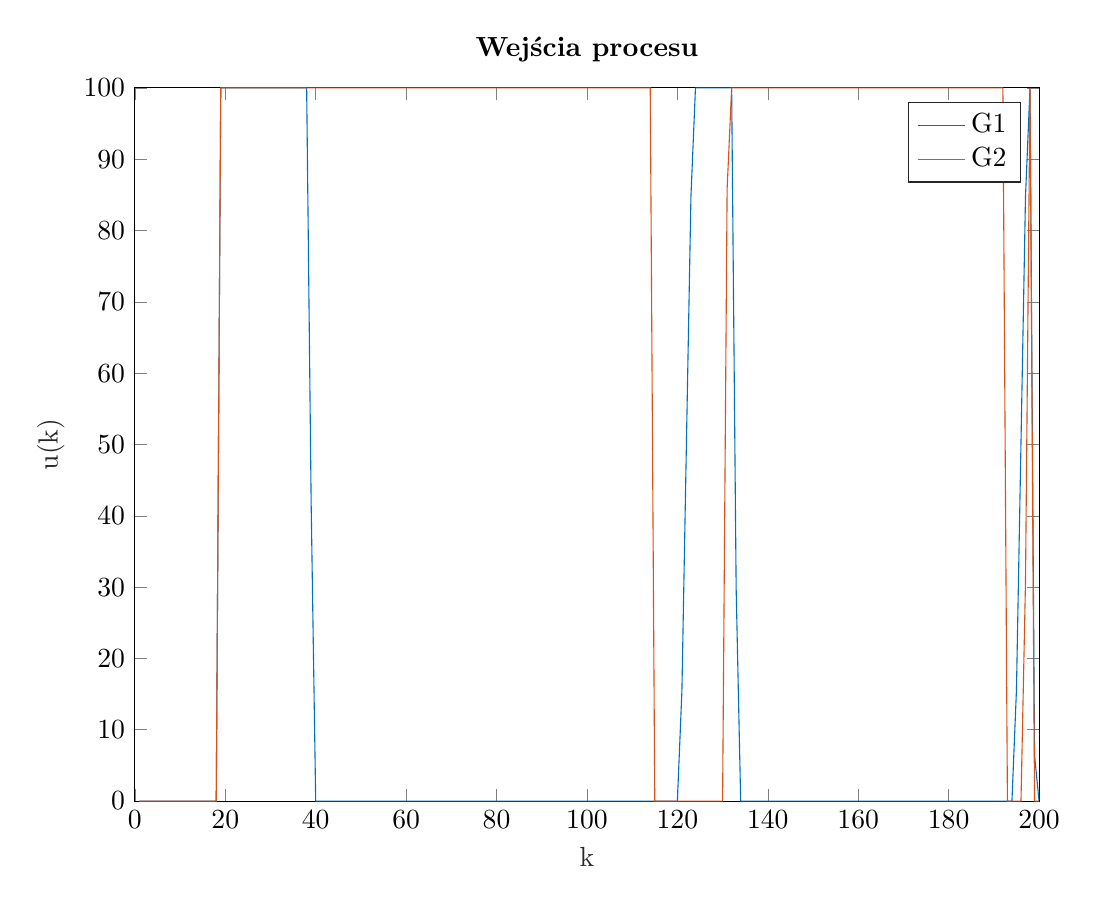
\begin{tikzpicture}

\begin{axis}[%
width=4.521in,
height=3.566in,
at={(0.758in,0.481in)},
scale only axis,
xmin=0,
xmax=200,
xlabel style={font=\color{white!15!black}},
xlabel={k},
ymin=0,
ymax=100,
ylabel style={font=\color{white!15!black}},
ylabel={u(k)},
axis background/.style={fill=white},
title style={font=\bfseries},
title={Wejścia procesu},
legend style={legend cell align=left, align=left, draw=white!15!black}
]
\addplot [color=mycolor1]
  table[row sep=crcr]{%
1	0\\
2	0\\
3	0\\
4	0\\
5	0\\
6	0\\
7	0\\
8	0\\
9	0\\
10	0\\
11	0\\
12	0\\
13	0\\
14	0\\
15	0\\
16	0\\
17	0\\
18	0\\
19	100\\
20	100\\
21	100\\
22	100\\
23	100\\
24	100\\
25	100\\
26	100\\
27	100\\
28	100\\
29	100\\
30	100\\
31	100\\
32	100\\
33	100\\
34	100\\
35	100\\
36	100\\
37	100\\
38	100\\
39	41.5\\
40	0\\
41	0\\
42	0\\
43	0\\
44	0\\
45	0\\
46	0\\
47	0\\
48	0\\
49	0\\
50	0\\
51	0\\
52	0\\
53	0\\
54	0\\
55	0\\
56	0\\
57	0\\
58	0\\
59	0\\
60	0\\
61	0\\
62	0\\
63	0\\
64	0\\
65	0\\
66	0\\
67	0\\
68	0\\
69	0\\
70	0\\
71	0\\
72	0\\
73	0\\
74	0\\
75	0\\
76	0\\
77	0\\
78	0\\
79	0\\
80	0\\
81	0\\
82	0\\
83	0\\
84	0\\
85	0\\
86	0\\
87	0\\
88	0\\
89	0\\
90	0\\
91	0\\
92	0\\
93	0\\
94	0\\
95	0\\
96	0\\
97	0\\
98	0\\
99	0\\
100	0\\
101	0\\
102	0\\
103	0\\
104	0\\
105	0\\
106	0\\
107	0\\
108	0\\
109	0\\
110	0\\
111	0\\
112	0\\
113	0\\
114	0\\
115	0\\
116	0\\
117	0\\
118	0\\
119	0\\
120	0\\
121	15.4\\
122	50.2\\
123	84.8\\
124	100\\
125	100\\
126	100\\
127	100\\
128	100\\
129	100\\
130	100\\
131	100\\
132	100\\
133	29.8\\
134	0\\
135	0\\
136	0\\
137	0\\
138	0\\
139	0\\
140	0\\
141	0\\
142	0\\
143	0\\
144	0\\
145	0\\
146	0\\
147	0\\
148	0\\
149	0\\
150	0\\
151	0\\
152	0\\
153	0\\
154	0\\
155	0\\
156	0\\
157	0\\
158	0\\
159	0\\
160	0\\
161	0\\
162	0\\
163	0\\
164	0\\
165	0\\
166	0\\
167	0\\
168	0\\
169	0\\
170	0\\
171	0\\
172	0\\
173	0\\
174	0\\
175	0\\
176	0\\
177	0\\
178	0\\
179	0\\
180	0\\
181	0\\
182	0\\
183	0\\
184	0\\
185	0\\
186	0\\
187	0\\
188	0\\
189	0\\
190	0\\
191	0\\
192	0\\
193	0\\
194	0\\
195	15.6\\
196	50.2\\
197	84.8\\
198	100\\
199	6.4\\
200	0\\
201	0\\
202	0\\
203	0\\
204	0\\
205	0\\
206	0\\
207	0\\
208	0\\
209	0\\
210	0\\
211	0\\
212	0\\
213	0\\
214	0\\
215	0\\
216	0\\
217	0\\
218	0\\
};
\addlegendentry{G1}

\addplot [color=mycolor2]
  table[row sep=crcr]{%
1	0\\
2	0\\
3	0\\
4	0\\
5	0\\
6	0\\
7	0\\
8	0\\
9	0\\
10	0\\
11	0\\
12	0\\
13	0\\
14	0\\
15	0\\
16	0\\
17	0\\
18	0\\
19	100\\
20	100\\
21	100\\
22	100\\
23	100\\
24	100\\
25	100\\
26	100\\
27	100\\
28	100\\
29	100\\
30	100\\
31	100\\
32	100\\
33	100\\
34	100\\
35	100\\
36	100\\
37	100\\
38	100\\
39	100\\
40	100\\
41	100\\
42	100\\
43	100\\
44	100\\
45	100\\
46	100\\
47	100\\
48	100\\
49	100\\
50	100\\
51	100\\
52	100\\
53	100\\
54	100\\
55	100\\
56	100\\
57	100\\
58	100\\
59	100\\
60	100\\
61	100\\
62	100\\
63	100\\
64	100\\
65	100\\
66	100\\
67	100\\
68	100\\
69	100\\
70	100\\
71	100\\
72	100\\
73	100\\
74	100\\
75	100\\
76	100\\
77	100\\
78	100\\
79	100\\
80	100\\
81	100\\
82	100\\
83	100\\
84	100\\
85	100\\
86	100\\
87	100\\
88	100\\
89	100\\
90	100\\
91	100\\
92	100\\
93	100\\
94	100\\
95	100\\
96	100\\
97	100\\
98	100\\
99	100\\
100	100\\
101	100\\
102	100\\
103	100\\
104	100\\
105	100\\
106	100\\
107	100\\
108	100\\
109	100\\
110	100\\
111	100\\
112	100\\
113	100\\
114	100\\
115	0\\
116	0\\
117	0\\
118	0\\
119	0\\
120	0\\
121	0\\
122	0\\
123	0\\
124	0\\
125	0\\
126	0\\
127	0\\
128	0\\
129	0\\
130	0\\
131	85.8\\
132	100\\
133	100\\
134	100\\
135	100\\
136	100\\
137	100\\
138	100\\
139	100\\
140	100\\
141	100\\
142	100\\
143	100\\
144	100\\
145	100\\
146	100\\
147	100\\
148	100\\
149	100\\
150	100\\
151	100\\
152	100\\
153	100\\
154	100\\
155	100\\
156	100\\
157	100\\
158	100\\
159	100\\
160	100\\
161	100\\
162	100\\
163	100\\
164	100\\
165	100\\
166	100\\
167	100\\
168	100\\
169	100\\
170	100\\
171	100\\
172	100\\
173	100\\
174	100\\
175	100\\
176	100\\
177	100\\
178	100\\
179	100\\
180	100\\
181	100\\
182	100\\
183	100\\
184	100\\
185	100\\
186	100\\
187	100\\
188	100\\
189	100\\
190	100\\
191	100\\
192	100\\
193	0\\
194	0\\
195	0\\
196	0\\
197	30.8\\
198	100\\
199	0\\
200	0\\
201	0\\
202	0\\
203	0\\
204	0\\
205	0\\
206	0\\
207	0\\
208	0\\
209	0\\
210	0\\
211	0\\
212	0\\
213	100\\
214	100\\
215	100\\
216	100\\
217	100\\
218	100\\
};
\addlegendentry{G2}

\end{axis}
\end{tikzpicture}%
\caption{Sygnały stejące: PID1: K=1 $T_i$=10 $T_d$=3 PID2: K=3 $T_i$=9 $T_d$=2}
\end{figure}

\begin{figure}[H]
\centering
% This file was created by matlab2tikz.
%
%The latest updates can be retrieved from
%  http://www.mathworks.com/matlabcentral/fileexchange/22022-matlab2tikz-matlab2tikz
%where you can also make suggestions and rate matlab2tikz.
%
\definecolor{mycolor1}{rgb}{0.00000,0.44700,0.74100}%
\definecolor{mycolor2}{rgb}{0.85000,0.32500,0.09800}%
\definecolor{mycolor3}{rgb}{0.92900,0.69400,0.12500}%
\definecolor{mycolor4}{rgb}{0.49400,0.18400,0.55600}%
%
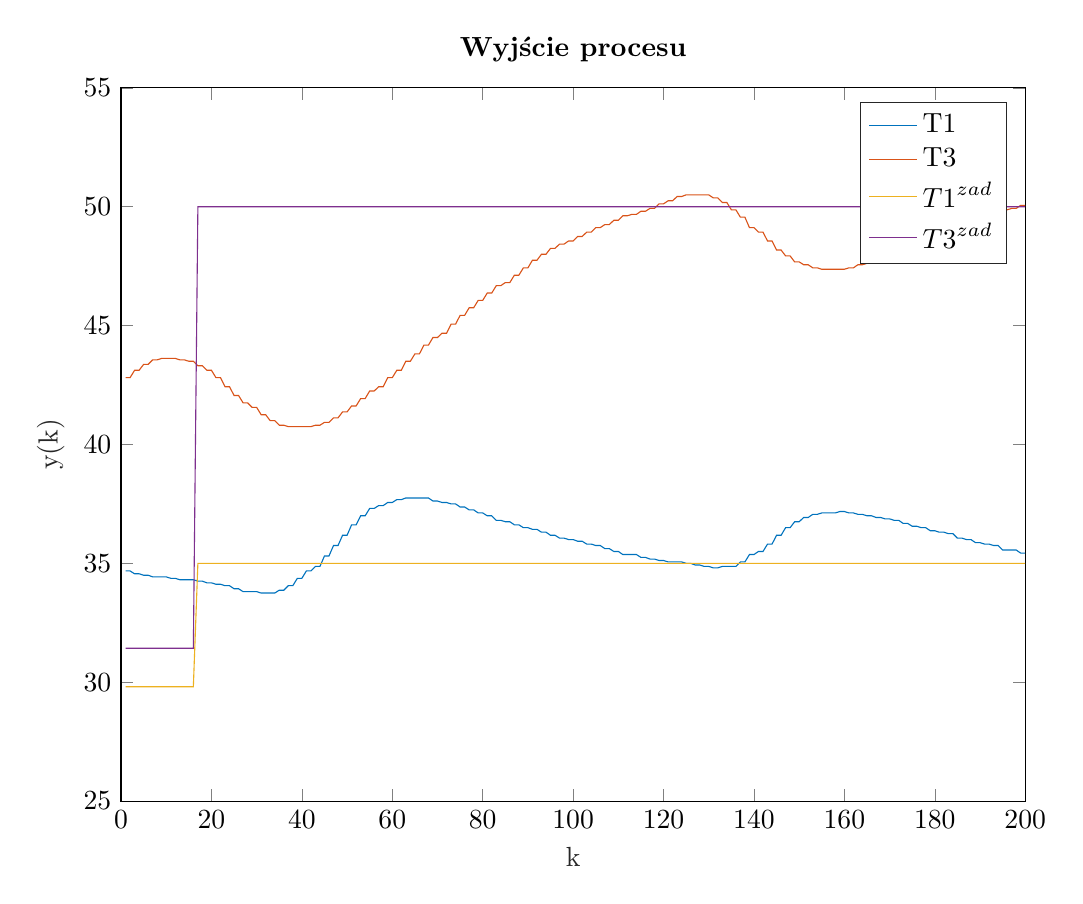
\begin{tikzpicture}

\begin{axis}[%
width=4.521in,
height=3.566in,
at={(0.758in,0.481in)},
scale only axis,
xmin=0,
xmax=200,
xlabel style={font=\color{white!15!black}},
xlabel={k},
ymin=25,
ymax=55,
ylabel style={font=\color{white!15!black}},
ylabel={y(k)},
axis background/.style={fill=white},
title style={font=\bfseries},
title={Wyjście procesu},
legend style={legend cell align=left, align=left, draw=white!15!black}
]
\addplot [color=mycolor1]
  table[row sep=crcr]{%
1	34.68\\
2	34.68\\
3	34.56\\
4	34.56\\
5	34.5\\
6	34.5\\
7	34.43\\
8	34.43\\
9	34.43\\
10	34.43\\
11	34.37\\
12	34.37\\
13	34.31\\
14	34.31\\
15	34.31\\
16	34.31\\
17	34.25\\
18	34.25\\
19	34.18\\
20	34.18\\
21	34.12\\
22	34.12\\
23	34.06\\
24	34.06\\
25	33.93\\
26	33.93\\
27	33.81\\
28	33.81\\
29	33.81\\
30	33.81\\
31	33.75\\
32	33.75\\
33	33.75\\
34	33.75\\
35	33.87\\
36	33.87\\
37	34.06\\
38	34.06\\
39	34.37\\
40	34.37\\
41	34.68\\
42	34.68\\
43	34.87\\
44	34.87\\
45	35.31\\
46	35.31\\
47	35.75\\
48	35.75\\
49	36.18\\
50	36.18\\
51	36.62\\
52	36.62\\
53	37\\
54	37\\
55	37.31\\
56	37.31\\
57	37.43\\
58	37.43\\
59	37.56\\
60	37.56\\
61	37.68\\
62	37.68\\
63	37.75\\
64	37.75\\
65	37.75\\
66	37.75\\
67	37.75\\
68	37.75\\
69	37.62\\
70	37.62\\
71	37.56\\
72	37.56\\
73	37.5\\
74	37.5\\
75	37.37\\
76	37.37\\
77	37.25\\
78	37.25\\
79	37.12\\
80	37.12\\
81	37\\
82	37\\
83	36.81\\
84	36.81\\
85	36.75\\
86	36.75\\
87	36.62\\
88	36.62\\
89	36.5\\
90	36.5\\
91	36.43\\
92	36.43\\
93	36.31\\
94	36.31\\
95	36.18\\
96	36.18\\
97	36.06\\
98	36.06\\
99	36\\
100	36\\
101	35.93\\
102	35.93\\
103	35.81\\
104	35.81\\
105	35.75\\
106	35.75\\
107	35.62\\
108	35.62\\
109	35.5\\
110	35.5\\
111	35.37\\
112	35.37\\
113	35.37\\
114	35.37\\
115	35.25\\
116	35.25\\
117	35.18\\
118	35.18\\
119	35.12\\
120	35.12\\
121	35.06\\
122	35.06\\
123	35.06\\
124	35.06\\
125	35\\
126	35\\
127	34.93\\
128	34.93\\
129	34.87\\
130	34.87\\
131	34.81\\
132	34.81\\
133	34.87\\
134	34.87\\
135	34.87\\
136	34.87\\
137	35.06\\
138	35.06\\
139	35.37\\
140	35.37\\
141	35.5\\
142	35.5\\
143	35.81\\
144	35.81\\
145	36.18\\
146	36.18\\
147	36.5\\
148	36.5\\
149	36.75\\
150	36.75\\
151	36.93\\
152	36.93\\
153	37.06\\
154	37.06\\
155	37.12\\
156	37.12\\
157	37.12\\
158	37.12\\
159	37.18\\
160	37.18\\
161	37.12\\
162	37.12\\
163	37.06\\
164	37.06\\
165	37\\
166	37\\
167	36.93\\
168	36.93\\
169	36.87\\
170	36.87\\
171	36.81\\
172	36.81\\
173	36.68\\
174	36.68\\
175	36.56\\
176	36.56\\
177	36.5\\
178	36.5\\
179	36.37\\
180	36.37\\
181	36.31\\
182	36.31\\
183	36.25\\
184	36.25\\
185	36.06\\
186	36.06\\
187	36\\
188	36\\
189	35.87\\
190	35.87\\
191	35.81\\
192	35.81\\
193	35.75\\
194	35.75\\
195	35.56\\
196	35.56\\
197	35.56\\
198	35.56\\
199	35.43\\
200	35.43\\
201	35.31\\
202	35.31\\
203	35.25\\
204	35.25\\
205	35.25\\
206	35.25\\
207	35.18\\
208	35.18\\
209	35.25\\
210	35.25\\
211	35.31\\
212	35.31\\
213	35.37\\
214	35.37\\
215	35.37\\
216	35.37\\
217	35.43\\
218	35.43\\
};
\addlegendentry{T1}

\addplot [color=mycolor2]
  table[row sep=crcr]{%
1	42.81\\
2	42.81\\
3	43.12\\
4	43.12\\
5	43.37\\
6	43.37\\
7	43.56\\
8	43.56\\
9	43.62\\
10	43.62\\
11	43.62\\
12	43.62\\
13	43.56\\
14	43.56\\
15	43.5\\
16	43.5\\
17	43.31\\
18	43.31\\
19	43.12\\
20	43.12\\
21	42.81\\
22	42.81\\
23	42.43\\
24	42.43\\
25	42.06\\
26	42.06\\
27	41.75\\
28	41.75\\
29	41.56\\
30	41.56\\
31	41.25\\
32	41.25\\
33	41\\
34	41\\
35	40.81\\
36	40.81\\
37	40.75\\
38	40.75\\
39	40.75\\
40	40.75\\
41	40.75\\
42	40.75\\
43	40.81\\
44	40.81\\
45	40.93\\
46	40.93\\
47	41.12\\
48	41.12\\
49	41.37\\
50	41.37\\
51	41.62\\
52	41.62\\
53	41.93\\
54	41.93\\
55	42.25\\
56	42.25\\
57	42.43\\
58	42.43\\
59	42.81\\
60	42.81\\
61	43.12\\
62	43.12\\
63	43.5\\
64	43.5\\
65	43.81\\
66	43.81\\
67	44.18\\
68	44.18\\
69	44.5\\
70	44.5\\
71	44.68\\
72	44.68\\
73	45.06\\
74	45.06\\
75	45.43\\
76	45.43\\
77	45.75\\
78	45.75\\
79	46.06\\
80	46.06\\
81	46.37\\
82	46.37\\
83	46.68\\
84	46.68\\
85	46.81\\
86	46.81\\
87	47.12\\
88	47.12\\
89	47.43\\
90	47.43\\
91	47.75\\
92	47.75\\
93	48\\
94	48\\
95	48.25\\
96	48.25\\
97	48.43\\
98	48.43\\
99	48.56\\
100	48.56\\
101	48.75\\
102	48.75\\
103	48.93\\
104	48.93\\
105	49.12\\
106	49.12\\
107	49.25\\
108	49.25\\
109	49.43\\
110	49.43\\
111	49.62\\
112	49.62\\
113	49.68\\
114	49.68\\
115	49.81\\
116	49.81\\
117	49.93\\
118	49.93\\
119	50.12\\
120	50.12\\
121	50.25\\
122	50.25\\
123	50.43\\
124	50.43\\
125	50.5\\
126	50.5\\
127	50.5\\
128	50.5\\
129	50.5\\
130	50.5\\
131	50.37\\
132	50.37\\
133	50.18\\
134	50.18\\
135	49.87\\
136	49.87\\
137	49.56\\
138	49.56\\
139	49.12\\
140	49.12\\
141	48.93\\
142	48.93\\
143	48.56\\
144	48.56\\
145	48.18\\
146	48.18\\
147	47.93\\
148	47.93\\
149	47.68\\
150	47.68\\
151	47.56\\
152	47.56\\
153	47.43\\
154	47.43\\
155	47.37\\
156	47.37\\
157	47.37\\
158	47.37\\
159	47.37\\
160	47.37\\
161	47.43\\
162	47.43\\
163	47.56\\
164	47.56\\
165	47.62\\
166	47.62\\
167	47.81\\
168	47.81\\
169	47.87\\
170	47.87\\
171	48\\
172	48\\
173	48.18\\
174	48.18\\
175	48.37\\
176	48.37\\
177	48.56\\
178	48.56\\
179	48.75\\
180	48.75\\
181	48.87\\
182	48.87\\
183	49\\
184	49\\
185	49.12\\
186	49.12\\
187	49.25\\
188	49.25\\
189	49.43\\
190	49.43\\
191	49.56\\
192	49.56\\
193	49.75\\
194	49.75\\
195	49.87\\
196	49.87\\
197	49.93\\
198	49.93\\
199	50.06\\
200	50.06\\
201	50.18\\
202	50.18\\
203	50.31\\
204	50.31\\
205	50.37\\
206	50.37\\
207	50.37\\
208	50.37\\
209	50.31\\
210	50.31\\
211	50.25\\
212	50.25\\
213	50.06\\
214	50.06\\
215	49.81\\
216	49.81\\
217	49.43\\
218	49.43\\
};
\addlegendentry{T3}

\addplot [color=mycolor3]
  table[row sep=crcr]{%
1	29.81\\
2	29.81\\
3	29.81\\
4	29.81\\
5	29.81\\
6	29.81\\
7	29.81\\
8	29.81\\
9	29.81\\
10	29.81\\
11	29.81\\
12	29.81\\
13	29.81\\
14	29.81\\
15	29.81\\
16	29.81\\
17	35\\
18	35\\
19	35\\
20	35\\
21	35\\
22	35\\
23	35\\
24	35\\
25	35\\
26	35\\
27	35\\
28	35\\
29	35\\
30	35\\
31	35\\
32	35\\
33	35\\
34	35\\
35	35\\
36	35\\
37	35\\
38	35\\
39	35\\
40	35\\
41	35\\
42	35\\
43	35\\
44	35\\
45	35\\
46	35\\
47	35\\
48	35\\
49	35\\
50	35\\
51	35\\
52	35\\
53	35\\
54	35\\
55	35\\
56	35\\
57	35\\
58	35\\
59	35\\
60	35\\
61	35\\
62	35\\
63	35\\
64	35\\
65	35\\
66	35\\
67	35\\
68	35\\
69	35\\
70	35\\
71	35\\
72	35\\
73	35\\
74	35\\
75	35\\
76	35\\
77	35\\
78	35\\
79	35\\
80	35\\
81	35\\
82	35\\
83	35\\
84	35\\
85	35\\
86	35\\
87	35\\
88	35\\
89	35\\
90	35\\
91	35\\
92	35\\
93	35\\
94	35\\
95	35\\
96	35\\
97	35\\
98	35\\
99	35\\
100	35\\
101	35\\
102	35\\
103	35\\
104	35\\
105	35\\
106	35\\
107	35\\
108	35\\
109	35\\
110	35\\
111	35\\
112	35\\
113	35\\
114	35\\
115	35\\
116	35\\
117	35\\
118	35\\
119	35\\
120	35\\
121	35\\
122	35\\
123	35\\
124	35\\
125	35\\
126	35\\
127	35\\
128	35\\
129	35\\
130	35\\
131	35\\
132	35\\
133	35\\
134	35\\
135	35\\
136	35\\
137	35\\
138	35\\
139	35\\
140	35\\
141	35\\
142	35\\
143	35\\
144	35\\
145	35\\
146	35\\
147	35\\
148	35\\
149	35\\
150	35\\
151	35\\
152	35\\
153	35\\
154	35\\
155	35\\
156	35\\
157	35\\
158	35\\
159	35\\
160	35\\
161	35\\
162	35\\
163	35\\
164	35\\
165	35\\
166	35\\
167	35\\
168	35\\
169	35\\
170	35\\
171	35\\
172	35\\
173	35\\
174	35\\
175	35\\
176	35\\
177	35\\
178	35\\
179	35\\
180	35\\
181	35\\
182	35\\
183	35\\
184	35\\
185	35\\
186	35\\
187	35\\
188	35\\
189	35\\
190	35\\
191	35\\
192	35\\
193	35\\
194	35\\
195	35\\
196	35\\
197	35\\
198	35\\
199	35\\
200	35\\
201	35\\
202	35\\
203	35\\
204	35\\
205	35\\
206	35\\
207	35\\
208	35\\
209	35\\
210	35\\
211	35\\
212	35\\
213	35\\
214	35\\
215	35\\
216	35\\
217	35\\
218	35\\
};
\addlegendentry{$\text{T1}^{\text{zad}}$}

\addplot [color=mycolor4]
  table[row sep=crcr]{%
1	31.43\\
2	31.43\\
3	31.43\\
4	31.43\\
5	31.43\\
6	31.43\\
7	31.43\\
8	31.43\\
9	31.43\\
10	31.43\\
11	31.43\\
12	31.43\\
13	31.43\\
14	31.43\\
15	31.43\\
16	31.43\\
17	50\\
18	50\\
19	50\\
20	50\\
21	50\\
22	50\\
23	50\\
24	50\\
25	50\\
26	50\\
27	50\\
28	50\\
29	50\\
30	50\\
31	50\\
32	50\\
33	50\\
34	50\\
35	50\\
36	50\\
37	50\\
38	50\\
39	50\\
40	50\\
41	50\\
42	50\\
43	50\\
44	50\\
45	50\\
46	50\\
47	50\\
48	50\\
49	50\\
50	50\\
51	50\\
52	50\\
53	50\\
54	50\\
55	50\\
56	50\\
57	50\\
58	50\\
59	50\\
60	50\\
61	50\\
62	50\\
63	50\\
64	50\\
65	50\\
66	50\\
67	50\\
68	50\\
69	50\\
70	50\\
71	50\\
72	50\\
73	50\\
74	50\\
75	50\\
76	50\\
77	50\\
78	50\\
79	50\\
80	50\\
81	50\\
82	50\\
83	50\\
84	50\\
85	50\\
86	50\\
87	50\\
88	50\\
89	50\\
90	50\\
91	50\\
92	50\\
93	50\\
94	50\\
95	50\\
96	50\\
97	50\\
98	50\\
99	50\\
100	50\\
101	50\\
102	50\\
103	50\\
104	50\\
105	50\\
106	50\\
107	50\\
108	50\\
109	50\\
110	50\\
111	50\\
112	50\\
113	50\\
114	50\\
115	50\\
116	50\\
117	50\\
118	50\\
119	50\\
120	50\\
121	50\\
122	50\\
123	50\\
124	50\\
125	50\\
126	50\\
127	50\\
128	50\\
129	50\\
130	50\\
131	50\\
132	50\\
133	50\\
134	50\\
135	50\\
136	50\\
137	50\\
138	50\\
139	50\\
140	50\\
141	50\\
142	50\\
143	50\\
144	50\\
145	50\\
146	50\\
147	50\\
148	50\\
149	50\\
150	50\\
151	50\\
152	50\\
153	50\\
154	50\\
155	50\\
156	50\\
157	50\\
158	50\\
159	50\\
160	50\\
161	50\\
162	50\\
163	50\\
164	50\\
165	50\\
166	50\\
167	50\\
168	50\\
169	50\\
170	50\\
171	50\\
172	50\\
173	50\\
174	50\\
175	50\\
176	50\\
177	50\\
178	50\\
179	50\\
180	50\\
181	50\\
182	50\\
183	50\\
184	50\\
185	50\\
186	50\\
187	50\\
188	50\\
189	50\\
190	50\\
191	50\\
192	50\\
193	50\\
194	50\\
195	50\\
196	50\\
197	50\\
198	50\\
199	50\\
200	50\\
201	50\\
202	50\\
203	50\\
204	50\\
205	50\\
206	50\\
207	50\\
208	50\\
209	50\\
210	50\\
211	50\\
212	50\\
213	50\\
214	50\\
215	50\\
216	50\\
217	50\\
218	50\\
};
\addlegendentry{$\text{T3}^{\text{zad}}$}

\end{axis}
\end{tikzpicture}%
\caption{Wyjścia obiektu: PID1: K=1 $T_i$=10 $T_d$=3 PID2: K=3 $T_i$=9 $T_d$=2}
\end{figure}


Żaden z powyższych zestawów regulatorów nie działa w sposób zadowalający. Sygnały wyjściowe zbliżają się do wartości zadanej, jednakże wartość ta ciągle oscyluje (oscylacje są dość duże). Rozwiązaniem tego problemu może być próba dostrojenia regulatorów.

%%%%%%%%%%%%%% Podpunkt4
\section{Regulator DMC}
Implementacja regulatora DMC w wersji 2x2 zaczeła się od wyznaczenia współczynników s. Do tego celu należy zebrać przebiegi wyjść na skok sygnału sterującego (kolejno skok na wejściu pierszym G1 przy stałym G2 oraz skok na wejściu G2 przy stałym G1). Następnie dla każdego z przebiegów należy zostosować wzór:
\begin{equation}
S_i=\frac{Y(i)-Y_{pp}}{\triangle U} \textrm{ ,dla } i=1,2 \ldots D
\label{step_norm}
\end{equation}

\begin{figure}[H]
\centering
% This file was created by matlab2tikz.
%
%The latest updates can be retrieved from
%  http://www.mathworks.com/matlabcentral/fileexchange/22022-matlab2tikz-matlab2tikz
%where you can also make suggestions and rate matlab2tikz.
%
\definecolor{mycolor1}{rgb}{0.00000,0.44700,0.74100}%
%
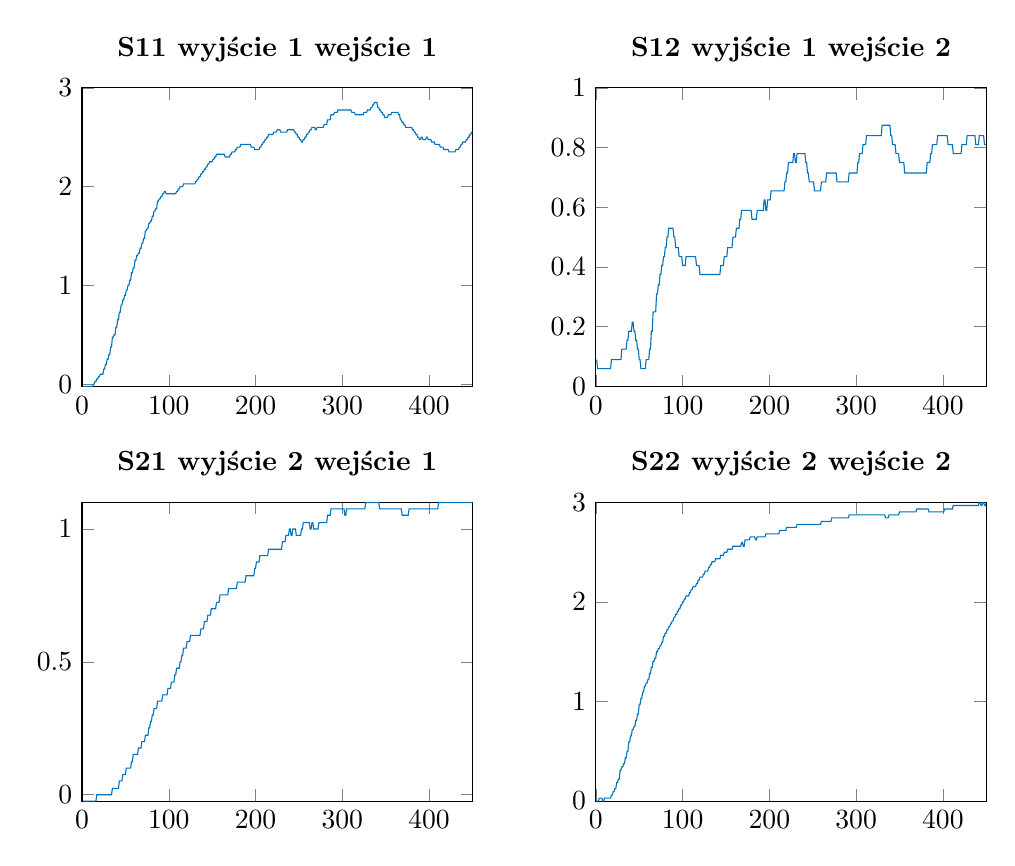
\begin{tikzpicture}

\begin{axis}[%
width=1.952in,
height=1.493in,
at={(0.758in,2.554in)},
scale only axis,
xmin=0,
xmax=450,
ymin=-0.024,
ymax=3,
axis background/.style={fill=white},
title style={font=\bfseries},
title={S11 wyjście 1 wejście 1}
]
\addplot [color=mycolor1, forget plot]
  table[row sep=crcr]{%
1	-0.024\\
2	-0.024\\
3	-0.024\\
4	-0.024\\
5	-0.024\\
6	-0.024\\
7	-0.024\\
8	-0.024\\
9	-0.024\\
10	-0.024\\
11	-0.024\\
12	-0.024\\
13	0\\
14	0\\
15	0.028\\
16	0.028\\
17	0.052\\
18	0.052\\
19	0.076\\
20	0.076\\
21	0.1\\
22	0.1\\
23	0.1\\
24	0.1\\
25	0.152\\
26	0.152\\
27	0.2\\
28	0.2\\
29	0.252\\
30	0.252\\
31	0.3\\
32	0.3\\
33	0.376\\
34	0.376\\
35	0.476\\
36	0.476\\
37	0.5\\
38	0.5\\
39	0.576\\
40	0.576\\
41	0.652\\
42	0.652\\
43	0.728\\
44	0.728\\
45	0.8\\
46	0.8\\
47	0.852\\
48	0.852\\
49	0.9\\
50	0.9\\
51	0.952\\
52	0.952\\
53	1\\
54	1\\
55	1.052\\
56	1.052\\
57	1.128\\
58	1.128\\
59	1.176\\
60	1.176\\
61	1.252\\
62	1.252\\
63	1.3\\
64	1.3\\
65	1.328\\
66	1.328\\
67	1.376\\
68	1.376\\
69	1.428\\
70	1.428\\
71	1.476\\
72	1.476\\
73	1.552\\
74	1.552\\
75	1.576\\
76	1.576\\
77	1.628\\
78	1.628\\
79	1.652\\
80	1.652\\
81	1.7\\
82	1.7\\
83	1.752\\
84	1.752\\
85	1.776\\
86	1.776\\
87	1.852\\
88	1.852\\
89	1.876\\
90	1.876\\
91	1.9\\
92	1.9\\
93	1.928\\
94	1.928\\
95	1.952\\
96	1.952\\
97	1.928\\
98	1.928\\
99	1.928\\
100	1.928\\
101	1.928\\
102	1.928\\
103	1.928\\
104	1.928\\
105	1.928\\
106	1.928\\
107	1.928\\
108	1.928\\
109	1.952\\
110	1.952\\
111	1.976\\
112	1.976\\
113	2\\
114	2\\
115	2\\
116	2\\
117	2.028\\
118	2.028\\
119	2.028\\
120	2.028\\
121	2.028\\
122	2.028\\
123	2.028\\
124	2.028\\
125	2.028\\
126	2.028\\
127	2.028\\
128	2.028\\
129	2.028\\
130	2.028\\
131	2.052\\
132	2.052\\
133	2.076\\
134	2.076\\
135	2.1\\
136	2.1\\
137	2.128\\
138	2.128\\
139	2.152\\
140	2.152\\
141	2.176\\
142	2.176\\
143	2.2\\
144	2.2\\
145	2.228\\
146	2.228\\
147	2.252\\
148	2.252\\
149	2.252\\
150	2.252\\
151	2.276\\
152	2.276\\
153	2.3\\
154	2.3\\
155	2.328\\
156	2.328\\
157	2.328\\
158	2.328\\
159	2.328\\
160	2.328\\
161	2.328\\
162	2.328\\
163	2.328\\
164	2.328\\
165	2.3\\
166	2.3\\
167	2.3\\
168	2.3\\
169	2.3\\
170	2.3\\
171	2.328\\
172	2.328\\
173	2.352\\
174	2.352\\
175	2.352\\
176	2.352\\
177	2.376\\
178	2.376\\
179	2.4\\
180	2.4\\
181	2.4\\
182	2.4\\
183	2.428\\
184	2.428\\
185	2.428\\
186	2.428\\
187	2.428\\
188	2.428\\
189	2.428\\
190	2.428\\
191	2.428\\
192	2.428\\
193	2.428\\
194	2.428\\
195	2.4\\
196	2.4\\
197	2.4\\
198	2.4\\
199	2.376\\
200	2.376\\
201	2.376\\
202	2.376\\
203	2.376\\
204	2.376\\
205	2.4\\
206	2.4\\
207	2.428\\
208	2.428\\
209	2.452\\
210	2.452\\
211	2.476\\
212	2.476\\
213	2.5\\
214	2.5\\
215	2.528\\
216	2.528\\
217	2.528\\
218	2.528\\
219	2.528\\
220	2.528\\
221	2.552\\
222	2.552\\
223	2.552\\
224	2.552\\
225	2.576\\
226	2.576\\
227	2.576\\
228	2.576\\
229	2.552\\
230	2.552\\
231	2.552\\
232	2.552\\
233	2.552\\
234	2.552\\
235	2.552\\
236	2.552\\
237	2.576\\
238	2.576\\
239	2.576\\
240	2.576\\
241	2.576\\
242	2.576\\
243	2.576\\
244	2.576\\
245	2.552\\
246	2.552\\
247	2.528\\
248	2.528\\
249	2.5\\
250	2.5\\
251	2.476\\
252	2.476\\
253	2.452\\
254	2.452\\
255	2.476\\
256	2.476\\
257	2.5\\
258	2.5\\
259	2.528\\
260	2.528\\
261	2.552\\
262	2.552\\
263	2.576\\
264	2.576\\
265	2.6\\
266	2.6\\
267	2.6\\
268	2.6\\
269	2.576\\
270	2.576\\
271	2.6\\
272	2.6\\
273	2.6\\
274	2.6\\
275	2.6\\
276	2.6\\
277	2.6\\
278	2.6\\
279	2.628\\
280	2.628\\
281	2.628\\
282	2.628\\
283	2.676\\
284	2.676\\
285	2.676\\
286	2.676\\
287	2.728\\
288	2.728\\
289	2.728\\
290	2.728\\
291	2.752\\
292	2.752\\
293	2.752\\
294	2.752\\
295	2.776\\
296	2.776\\
297	2.776\\
298	2.776\\
299	2.776\\
300	2.776\\
301	2.776\\
302	2.776\\
303	2.776\\
304	2.776\\
305	2.776\\
306	2.776\\
307	2.776\\
308	2.776\\
309	2.776\\
310	2.776\\
311	2.752\\
312	2.752\\
313	2.752\\
314	2.752\\
315	2.728\\
316	2.728\\
317	2.728\\
318	2.728\\
319	2.728\\
320	2.728\\
321	2.728\\
322	2.728\\
323	2.728\\
324	2.728\\
325	2.752\\
326	2.752\\
327	2.752\\
328	2.752\\
329	2.776\\
330	2.776\\
331	2.776\\
332	2.776\\
333	2.8\\
334	2.8\\
335	2.828\\
336	2.828\\
337	2.852\\
338	2.852\\
339	2.852\\
340	2.852\\
341	2.8\\
342	2.8\\
343	2.776\\
344	2.776\\
345	2.752\\
346	2.752\\
347	2.728\\
348	2.728\\
349	2.7\\
350	2.7\\
351	2.7\\
352	2.7\\
353	2.728\\
354	2.728\\
355	2.728\\
356	2.728\\
357	2.752\\
358	2.752\\
359	2.752\\
360	2.752\\
361	2.752\\
362	2.752\\
363	2.752\\
364	2.752\\
365	2.728\\
366	2.728\\
367	2.676\\
368	2.676\\
369	2.652\\
370	2.652\\
371	2.628\\
372	2.628\\
373	2.6\\
374	2.6\\
375	2.6\\
376	2.6\\
377	2.6\\
378	2.6\\
379	2.6\\
380	2.6\\
381	2.576\\
382	2.576\\
383	2.552\\
384	2.552\\
385	2.528\\
386	2.528\\
387	2.5\\
388	2.5\\
389	2.476\\
390	2.476\\
391	2.5\\
392	2.5\\
393	2.476\\
394	2.476\\
395	2.476\\
396	2.476\\
397	2.5\\
398	2.5\\
399	2.476\\
400	2.476\\
401	2.476\\
402	2.476\\
403	2.452\\
404	2.452\\
405	2.452\\
406	2.452\\
407	2.428\\
408	2.428\\
409	2.428\\
410	2.428\\
411	2.428\\
412	2.428\\
413	2.4\\
414	2.4\\
415	2.4\\
416	2.4\\
417	2.376\\
418	2.376\\
419	2.376\\
420	2.376\\
421	2.376\\
422	2.376\\
423	2.352\\
424	2.352\\
425	2.352\\
426	2.352\\
427	2.352\\
428	2.352\\
429	2.352\\
430	2.352\\
431	2.376\\
432	2.376\\
433	2.376\\
434	2.376\\
435	2.4\\
436	2.4\\
437	2.428\\
438	2.428\\
439	2.452\\
440	2.452\\
441	2.452\\
442	2.452\\
443	2.476\\
444	2.476\\
445	2.5\\
446	2.5\\
447	2.528\\
448	2.528\\
449	2.552\\
450	2.552\\
451	2.576\\
452	2.576\\
453	2.6\\
454	2.6\\
455	2.628\\
456	2.628\\
457	2.628\\
458	2.628\\
459	2.628\\
460	2.628\\
461	2.628\\
462	2.628\\
463	2.628\\
464	2.628\\
465	2.628\\
466	2.628\\
467	2.652\\
468	2.652\\
469	2.652\\
470	2.652\\
471	2.676\\
472	2.676\\
473	2.676\\
474	2.676\\
475	2.7\\
476	2.7\\
477	2.7\\
478	2.7\\
479	2.728\\
480	2.728\\
481	2.728\\
482	2.728\\
483	2.752\\
484	2.752\\
485	2.728\\
486	2.728\\
487	2.728\\
};
\end{axis}

\begin{axis}[%
width=1.952in,
height=1.493in,
at={(3.327in,0.481in)},
scale only axis,
xmin=0,
xmax=450,
ymin=0,
ymax=3,
axis background/.style={fill=white},
title style={font=\bfseries},
title={S22 wyjście 2 wejście 2}
]
\addplot [color=mycolor1, forget plot]
  table[row sep=crcr]{%
1	0\\
2	0\\
3	0\\
4	0.03\\
5	0.03\\
6	0.03\\
7	0.03\\
8	0\\
9	0\\
10	0.03\\
11	0.03\\
12	0.03\\
13	0.03\\
14	0.03\\
15	0.03\\
16	0.03\\
17	0.03\\
18	0.06\\
19	0.06\\
20	0.095\\
21	0.095\\
22	0.125\\
23	0.125\\
24	0.185\\
25	0.185\\
26	0.22\\
27	0.22\\
28	0.31\\
29	0.31\\
30	0.345\\
31	0.345\\
32	0.375\\
33	0.375\\
34	0.435\\
35	0.435\\
36	0.5\\
37	0.5\\
38	0.595\\
39	0.595\\
40	0.655\\
41	0.655\\
42	0.72\\
43	0.72\\
44	0.75\\
45	0.75\\
46	0.81\\
47	0.81\\
48	0.875\\
49	0.875\\
50	0.97\\
51	0.97\\
52	1.03\\
53	1.03\\
54	1.095\\
55	1.095\\
56	1.155\\
57	1.155\\
58	1.185\\
59	1.185\\
60	1.22\\
61	1.22\\
62	1.28\\
63	1.28\\
64	1.345\\
65	1.345\\
66	1.405\\
67	1.405\\
68	1.435\\
69	1.435\\
70	1.5\\
71	1.5\\
72	1.53\\
73	1.53\\
74	1.56\\
75	1.56\\
76	1.595\\
77	1.595\\
78	1.655\\
79	1.655\\
80	1.685\\
81	1.685\\
82	1.72\\
83	1.72\\
84	1.75\\
85	1.75\\
86	1.78\\
87	1.78\\
88	1.81\\
89	1.81\\
90	1.845\\
91	1.845\\
92	1.875\\
93	1.875\\
94	1.905\\
95	1.905\\
96	1.935\\
97	1.935\\
98	1.97\\
99	1.97\\
100	2\\
101	2\\
102	2.03\\
103	2.03\\
104	2.06\\
105	2.06\\
106	2.06\\
107	2.06\\
108	2.095\\
109	2.095\\
110	2.125\\
111	2.125\\
112	2.155\\
113	2.155\\
114	2.155\\
115	2.155\\
116	2.185\\
117	2.185\\
118	2.22\\
119	2.22\\
120	2.25\\
121	2.25\\
122	2.25\\
123	2.25\\
124	2.28\\
125	2.28\\
126	2.31\\
127	2.31\\
128	2.31\\
129	2.31\\
130	2.345\\
131	2.345\\
132	2.375\\
133	2.375\\
134	2.405\\
135	2.405\\
136	2.405\\
137	2.405\\
138	2.435\\
139	2.435\\
140	2.435\\
141	2.435\\
142	2.435\\
143	2.435\\
144	2.47\\
145	2.47\\
146	2.47\\
147	2.47\\
148	2.5\\
149	2.5\\
150	2.5\\
151	2.5\\
152	2.53\\
153	2.53\\
154	2.53\\
155	2.53\\
156	2.53\\
157	2.53\\
158	2.56\\
159	2.56\\
160	2.56\\
161	2.56\\
162	2.56\\
163	2.56\\
164	2.56\\
165	2.56\\
166	2.56\\
167	2.56\\
168	2.595\\
169	2.595\\
170	2.56\\
171	2.56\\
172	2.625\\
173	2.625\\
174	2.625\\
175	2.625\\
176	2.625\\
177	2.625\\
178	2.655\\
179	2.655\\
180	2.655\\
181	2.655\\
182	2.655\\
183	2.655\\
184	2.625\\
185	2.625\\
186	2.655\\
187	2.655\\
188	2.655\\
189	2.655\\
190	2.655\\
191	2.655\\
192	2.655\\
193	2.655\\
194	2.655\\
195	2.655\\
196	2.685\\
197	2.685\\
198	2.685\\
199	2.685\\
200	2.685\\
201	2.685\\
202	2.685\\
203	2.685\\
204	2.685\\
205	2.685\\
206	2.685\\
207	2.685\\
208	2.685\\
209	2.685\\
210	2.685\\
211	2.685\\
212	2.72\\
213	2.72\\
214	2.72\\
215	2.72\\
216	2.72\\
217	2.72\\
218	2.72\\
219	2.72\\
220	2.75\\
221	2.75\\
222	2.75\\
223	2.75\\
224	2.75\\
225	2.75\\
226	2.75\\
227	2.75\\
228	2.75\\
229	2.75\\
230	2.75\\
231	2.75\\
232	2.78\\
233	2.78\\
234	2.78\\
235	2.78\\
236	2.78\\
237	2.78\\
238	2.78\\
239	2.78\\
240	2.78\\
241	2.78\\
242	2.78\\
243	2.78\\
244	2.78\\
245	2.78\\
246	2.78\\
247	2.78\\
248	2.78\\
249	2.78\\
250	2.78\\
251	2.78\\
252	2.78\\
253	2.78\\
254	2.78\\
255	2.78\\
256	2.78\\
257	2.78\\
258	2.78\\
259	2.78\\
260	2.81\\
261	2.81\\
262	2.81\\
263	2.81\\
264	2.81\\
265	2.81\\
266	2.81\\
267	2.81\\
268	2.81\\
269	2.81\\
270	2.81\\
271	2.81\\
272	2.845\\
273	2.845\\
274	2.845\\
275	2.845\\
276	2.845\\
277	2.845\\
278	2.845\\
279	2.845\\
280	2.845\\
281	2.845\\
282	2.845\\
283	2.845\\
284	2.845\\
285	2.845\\
286	2.845\\
287	2.845\\
288	2.845\\
289	2.845\\
290	2.845\\
291	2.845\\
292	2.875\\
293	2.875\\
294	2.875\\
295	2.875\\
296	2.875\\
297	2.875\\
298	2.875\\
299	2.875\\
300	2.875\\
301	2.875\\
302	2.875\\
303	2.875\\
304	2.875\\
305	2.875\\
306	2.875\\
307	2.875\\
308	2.875\\
309	2.875\\
310	2.875\\
311	2.875\\
312	2.875\\
313	2.875\\
314	2.875\\
315	2.875\\
316	2.875\\
317	2.875\\
318	2.875\\
319	2.875\\
320	2.875\\
321	2.875\\
322	2.875\\
323	2.875\\
324	2.875\\
325	2.875\\
326	2.875\\
327	2.875\\
328	2.875\\
329	2.875\\
330	2.875\\
331	2.875\\
332	2.875\\
333	2.875\\
334	2.845\\
335	2.845\\
336	2.845\\
337	2.845\\
338	2.875\\
339	2.875\\
340	2.875\\
341	2.875\\
342	2.875\\
343	2.875\\
344	2.875\\
345	2.875\\
346	2.875\\
347	2.875\\
348	2.875\\
349	2.875\\
350	2.905\\
351	2.905\\
352	2.905\\
353	2.905\\
354	2.905\\
355	2.905\\
356	2.905\\
357	2.905\\
358	2.905\\
359	2.905\\
360	2.905\\
361	2.905\\
362	2.905\\
363	2.905\\
364	2.905\\
365	2.905\\
366	2.905\\
367	2.905\\
368	2.905\\
369	2.905\\
370	2.935\\
371	2.935\\
372	2.935\\
373	2.935\\
374	2.935\\
375	2.935\\
376	2.935\\
377	2.935\\
378	2.935\\
379	2.935\\
380	2.935\\
381	2.935\\
382	2.935\\
383	2.935\\
384	2.905\\
385	2.905\\
386	2.905\\
387	2.905\\
388	2.905\\
389	2.905\\
390	2.905\\
391	2.905\\
392	2.905\\
393	2.905\\
394	2.905\\
395	2.905\\
396	2.905\\
397	2.905\\
398	2.905\\
399	2.905\\
400	2.905\\
401	2.905\\
402	2.935\\
403	2.935\\
404	2.935\\
405	2.935\\
406	2.935\\
407	2.935\\
408	2.935\\
409	2.935\\
410	2.935\\
411	2.935\\
412	2.97\\
413	2.97\\
414	2.97\\
415	2.97\\
416	2.97\\
417	2.97\\
418	2.97\\
419	2.97\\
420	2.97\\
421	2.97\\
422	2.97\\
423	2.97\\
424	2.97\\
425	2.97\\
426	2.97\\
427	2.97\\
428	2.97\\
429	2.97\\
430	2.97\\
431	2.97\\
432	2.97\\
433	2.97\\
434	2.97\\
435	2.97\\
436	2.97\\
437	2.97\\
438	2.97\\
439	2.97\\
440	2.97\\
441	2.97\\
442	3\\
443	3\\
444	2.97\\
445	2.97\\
446	3\\
447	3\\
448	2.97\\
449	2.97\\
450	3\\
451	3\\
452	2.97\\
453	2.97\\
454	2.97\\
455	2.97\\
456	2.97\\
457	2.97\\
458	2.97\\
459	2.97\\
460	2.97\\
461	2.97\\
462	2.97\\
463	2.97\\
464	2.97\\
465	2.97\\
466	2.97\\
467	2.97\\
468	2.97\\
469	2.97\\
470	2.97\\
471	2.97\\
472	2.97\\
473	2.97\\
474	2.97\\
475	2.97\\
476	2.97\\
477	2.97\\
478	2.97\\
479	2.97\\
480	2.97\\
481	2.97\\
482	2.97\\
483	2.97\\
484	2.97\\
485	2.97\\
486	3\\
487	3\\
};
\end{axis}

\begin{axis}[%
width=1.952in,
height=1.493in,
at={(3.327in,2.554in)},
scale only axis,
xmin=0,
xmax=450,
ymin=0,
ymax=1,
axis background/.style={fill=white},
title style={font=\bfseries},
title={S12 wyjście 1 wejście 2}
]
\addplot [color=mycolor1, forget plot]
  table[row sep=crcr]{%
1	0.09\\
2	0.06\\
3	0.06\\
4	0.06\\
5	0.06\\
6	0.06\\
7	0.06\\
8	0.06\\
9	0.06\\
10	0.06\\
11	0.06\\
12	0.06\\
13	0.06\\
14	0.06\\
15	0.06\\
16	0.06\\
17	0.06\\
18	0.09\\
19	0.09\\
20	0.09\\
21	0.09\\
22	0.09\\
23	0.09\\
24	0.09\\
25	0.09\\
26	0.09\\
27	0.09\\
28	0.09\\
29	0.09\\
30	0.125\\
31	0.125\\
32	0.125\\
33	0.125\\
34	0.125\\
35	0.125\\
36	0.155\\
37	0.155\\
38	0.185\\
39	0.185\\
40	0.185\\
41	0.185\\
42	0.215\\
43	0.215\\
44	0.185\\
45	0.185\\
46	0.155\\
47	0.155\\
48	0.125\\
49	0.125\\
50	0.09\\
51	0.09\\
52	0.06\\
53	0.06\\
54	0.06\\
55	0.06\\
56	0.06\\
57	0.06\\
58	0.09\\
59	0.09\\
60	0.09\\
61	0.09\\
62	0.125\\
63	0.125\\
64	0.185\\
65	0.185\\
66	0.25\\
67	0.25\\
68	0.25\\
69	0.25\\
70	0.31\\
71	0.31\\
72	0.34\\
73	0.34\\
74	0.375\\
75	0.375\\
76	0.405\\
77	0.405\\
78	0.435\\
79	0.435\\
80	0.465\\
81	0.465\\
82	0.5\\
83	0.5\\
84	0.53\\
85	0.53\\
86	0.53\\
87	0.53\\
88	0.53\\
89	0.53\\
90	0.5\\
91	0.5\\
92	0.465\\
93	0.465\\
94	0.465\\
95	0.465\\
96	0.435\\
97	0.435\\
98	0.435\\
99	0.435\\
100	0.405\\
101	0.405\\
102	0.405\\
103	0.405\\
104	0.435\\
105	0.435\\
106	0.435\\
107	0.435\\
108	0.435\\
109	0.435\\
110	0.435\\
111	0.435\\
112	0.435\\
113	0.435\\
114	0.435\\
115	0.435\\
116	0.405\\
117	0.405\\
118	0.405\\
119	0.405\\
120	0.375\\
121	0.375\\
122	0.375\\
123	0.375\\
124	0.375\\
125	0.375\\
126	0.375\\
127	0.375\\
128	0.375\\
129	0.375\\
130	0.375\\
131	0.375\\
132	0.375\\
133	0.375\\
134	0.375\\
135	0.375\\
136	0.375\\
137	0.375\\
138	0.375\\
139	0.375\\
140	0.375\\
141	0.375\\
142	0.375\\
143	0.375\\
144	0.405\\
145	0.405\\
146	0.405\\
147	0.405\\
148	0.435\\
149	0.435\\
150	0.435\\
151	0.435\\
152	0.465\\
153	0.465\\
154	0.465\\
155	0.465\\
156	0.465\\
157	0.465\\
158	0.5\\
159	0.5\\
160	0.5\\
161	0.5\\
162	0.53\\
163	0.53\\
164	0.53\\
165	0.53\\
166	0.56\\
167	0.56\\
168	0.59\\
169	0.59\\
170	0.59\\
171	0.59\\
172	0.59\\
173	0.59\\
174	0.59\\
175	0.59\\
176	0.59\\
177	0.59\\
178	0.59\\
179	0.59\\
180	0.56\\
181	0.56\\
182	0.56\\
183	0.56\\
184	0.56\\
185	0.56\\
186	0.59\\
187	0.59\\
188	0.59\\
189	0.59\\
190	0.59\\
191	0.59\\
192	0.59\\
193	0.59\\
194	0.625\\
195	0.625\\
196	0.59\\
197	0.59\\
198	0.625\\
199	0.625\\
200	0.625\\
201	0.625\\
202	0.655\\
203	0.655\\
204	0.655\\
205	0.655\\
206	0.655\\
207	0.655\\
208	0.655\\
209	0.655\\
210	0.655\\
211	0.655\\
212	0.655\\
213	0.655\\
214	0.655\\
215	0.655\\
216	0.655\\
217	0.655\\
218	0.685\\
219	0.685\\
220	0.715\\
221	0.715\\
222	0.75\\
223	0.75\\
224	0.75\\
225	0.75\\
226	0.75\\
227	0.75\\
228	0.78\\
229	0.78\\
230	0.75\\
231	0.75\\
232	0.78\\
233	0.78\\
234	0.78\\
235	0.78\\
236	0.78\\
237	0.78\\
238	0.78\\
239	0.78\\
240	0.78\\
241	0.78\\
242	0.75\\
243	0.75\\
244	0.715\\
245	0.715\\
246	0.685\\
247	0.685\\
248	0.685\\
249	0.685\\
250	0.685\\
251	0.685\\
252	0.655\\
253	0.655\\
254	0.655\\
255	0.655\\
256	0.655\\
257	0.655\\
258	0.655\\
259	0.655\\
260	0.685\\
261	0.685\\
262	0.685\\
263	0.685\\
264	0.685\\
265	0.685\\
266	0.715\\
267	0.715\\
268	0.715\\
269	0.715\\
270	0.715\\
271	0.715\\
272	0.715\\
273	0.715\\
274	0.715\\
275	0.715\\
276	0.715\\
277	0.715\\
278	0.685\\
279	0.685\\
280	0.685\\
281	0.685\\
282	0.685\\
283	0.685\\
284	0.685\\
285	0.685\\
286	0.685\\
287	0.685\\
288	0.685\\
289	0.685\\
290	0.685\\
291	0.685\\
292	0.715\\
293	0.715\\
294	0.715\\
295	0.715\\
296	0.715\\
297	0.715\\
298	0.715\\
299	0.715\\
300	0.715\\
301	0.715\\
302	0.75\\
303	0.75\\
304	0.78\\
305	0.78\\
306	0.78\\
307	0.78\\
308	0.81\\
309	0.81\\
310	0.81\\
311	0.81\\
312	0.84\\
313	0.84\\
314	0.84\\
315	0.84\\
316	0.84\\
317	0.84\\
318	0.84\\
319	0.84\\
320	0.84\\
321	0.84\\
322	0.84\\
323	0.84\\
324	0.84\\
325	0.84\\
326	0.84\\
327	0.84\\
328	0.84\\
329	0.84\\
330	0.875\\
331	0.875\\
332	0.875\\
333	0.875\\
334	0.875\\
335	0.875\\
336	0.875\\
337	0.875\\
338	0.875\\
339	0.875\\
340	0.84\\
341	0.84\\
342	0.81\\
343	0.81\\
344	0.81\\
345	0.81\\
346	0.78\\
347	0.78\\
348	0.78\\
349	0.78\\
350	0.75\\
351	0.75\\
352	0.75\\
353	0.75\\
354	0.75\\
355	0.75\\
356	0.715\\
357	0.715\\
358	0.715\\
359	0.715\\
360	0.715\\
361	0.715\\
362	0.715\\
363	0.715\\
364	0.715\\
365	0.715\\
366	0.715\\
367	0.715\\
368	0.715\\
369	0.715\\
370	0.715\\
371	0.715\\
372	0.715\\
373	0.715\\
374	0.715\\
375	0.715\\
376	0.715\\
377	0.715\\
378	0.715\\
379	0.715\\
380	0.715\\
381	0.715\\
382	0.75\\
383	0.75\\
384	0.75\\
385	0.75\\
386	0.78\\
387	0.78\\
388	0.81\\
389	0.81\\
390	0.81\\
391	0.81\\
392	0.81\\
393	0.81\\
394	0.84\\
395	0.84\\
396	0.84\\
397	0.84\\
398	0.84\\
399	0.84\\
400	0.84\\
401	0.84\\
402	0.84\\
403	0.84\\
404	0.84\\
405	0.84\\
406	0.81\\
407	0.81\\
408	0.81\\
409	0.81\\
410	0.81\\
411	0.81\\
412	0.78\\
413	0.78\\
414	0.78\\
415	0.78\\
416	0.78\\
417	0.78\\
418	0.78\\
419	0.78\\
420	0.78\\
421	0.78\\
422	0.81\\
423	0.81\\
424	0.81\\
425	0.81\\
426	0.81\\
427	0.81\\
428	0.84\\
429	0.84\\
430	0.84\\
431	0.84\\
432	0.84\\
433	0.84\\
434	0.84\\
435	0.84\\
436	0.84\\
437	0.84\\
438	0.81\\
439	0.81\\
440	0.81\\
441	0.81\\
442	0.84\\
443	0.84\\
444	0.84\\
445	0.84\\
446	0.84\\
447	0.84\\
448	0.81\\
449	0.81\\
450	0.81\\
451	0.81\\
452	0.81\\
453	0.81\\
454	0.84\\
455	0.84\\
456	0.84\\
457	0.84\\
458	0.81\\
459	0.81\\
460	0.81\\
461	0.81\\
462	0.81\\
463	0.81\\
464	0.78\\
465	0.78\\
466	0.81\\
467	0.81\\
468	0.84\\
469	0.84\\
470	0.81\\
471	0.81\\
472	0.84\\
473	0.84\\
474	0.81\\
475	0.81\\
476	0.84\\
477	0.84\\
478	0.84\\
479	0.84\\
480	0.84\\
481	0.84\\
482	0.84\\
483	0.84\\
484	0.84\\
485	0.84\\
486	0.81\\
487	0.81\\
};
\end{axis}

\begin{axis}[%
width=1.952in,
height=1.493in,
at={(0.758in,0.481in)},
scale only axis,
xmin=0,
xmax=450,
ymin=-0.024,
ymax=1.1,
axis background/.style={fill=white},
title style={font=\bfseries},
title={S21 wyjście 2 wejście 1}
]
\addplot [color=mycolor1, forget plot]
  table[row sep=crcr]{%
1	-0.024\\
2	-0.024\\
3	-0.024\\
4	-0.024\\
5	-0.024\\
6	-0.024\\
7	-0.024\\
8	-0.024\\
9	-0.024\\
10	-0.024\\
11	-0.024\\
12	-0.024\\
13	-0.024\\
14	-0.024\\
15	-0.024\\
16	-0.024\\
17	0\\
18	0\\
19	0\\
20	0\\
21	0\\
22	0\\
23	0\\
24	0\\
25	0\\
26	0\\
27	0\\
28	0\\
29	0\\
30	0\\
31	0\\
32	0\\
33	0\\
34	0\\
35	0.024\\
36	0.024\\
37	0.024\\
38	0.024\\
39	0.024\\
40	0.024\\
41	0.024\\
42	0.024\\
43	0.052\\
44	0.052\\
45	0.052\\
46	0.052\\
47	0.076\\
48	0.076\\
49	0.076\\
50	0.076\\
51	0.1\\
52	0.1\\
53	0.1\\
54	0.1\\
55	0.1\\
56	0.1\\
57	0.124\\
58	0.124\\
59	0.152\\
60	0.152\\
61	0.152\\
62	0.152\\
63	0.152\\
64	0.152\\
65	0.176\\
66	0.176\\
67	0.176\\
68	0.176\\
69	0.2\\
70	0.2\\
71	0.2\\
72	0.2\\
73	0.224\\
74	0.224\\
75	0.224\\
76	0.224\\
77	0.252\\
78	0.252\\
79	0.276\\
80	0.276\\
81	0.3\\
82	0.3\\
83	0.324\\
84	0.324\\
85	0.324\\
86	0.324\\
87	0.352\\
88	0.352\\
89	0.352\\
90	0.352\\
91	0.352\\
92	0.352\\
93	0.376\\
94	0.376\\
95	0.376\\
96	0.376\\
97	0.376\\
98	0.376\\
99	0.4\\
100	0.4\\
101	0.4\\
102	0.4\\
103	0.424\\
104	0.424\\
105	0.424\\
106	0.424\\
107	0.452\\
108	0.452\\
109	0.476\\
110	0.476\\
111	0.476\\
112	0.476\\
113	0.5\\
114	0.5\\
115	0.524\\
116	0.524\\
117	0.552\\
118	0.552\\
119	0.552\\
120	0.552\\
121	0.576\\
122	0.576\\
123	0.576\\
124	0.576\\
125	0.6\\
126	0.6\\
127	0.6\\
128	0.6\\
129	0.6\\
130	0.6\\
131	0.6\\
132	0.6\\
133	0.6\\
134	0.6\\
135	0.6\\
136	0.6\\
137	0.624\\
138	0.624\\
139	0.624\\
140	0.624\\
141	0.652\\
142	0.652\\
143	0.652\\
144	0.652\\
145	0.676\\
146	0.676\\
147	0.676\\
148	0.676\\
149	0.7\\
150	0.7\\
151	0.7\\
152	0.7\\
153	0.7\\
154	0.7\\
155	0.724\\
156	0.724\\
157	0.724\\
158	0.724\\
159	0.752\\
160	0.752\\
161	0.752\\
162	0.752\\
163	0.752\\
164	0.752\\
165	0.752\\
166	0.752\\
167	0.752\\
168	0.752\\
169	0.776\\
170	0.776\\
171	0.776\\
172	0.776\\
173	0.776\\
174	0.776\\
175	0.776\\
176	0.776\\
177	0.776\\
178	0.776\\
179	0.8\\
180	0.8\\
181	0.8\\
182	0.8\\
183	0.8\\
184	0.8\\
185	0.8\\
186	0.8\\
187	0.8\\
188	0.8\\
189	0.824\\
190	0.824\\
191	0.824\\
192	0.824\\
193	0.824\\
194	0.824\\
195	0.824\\
196	0.824\\
197	0.824\\
198	0.824\\
199	0.852\\
200	0.852\\
201	0.876\\
202	0.876\\
203	0.876\\
204	0.876\\
205	0.9\\
206	0.9\\
207	0.9\\
208	0.9\\
209	0.9\\
210	0.9\\
211	0.9\\
212	0.9\\
213	0.9\\
214	0.9\\
215	0.924\\
216	0.924\\
217	0.924\\
218	0.924\\
219	0.924\\
220	0.924\\
221	0.924\\
222	0.924\\
223	0.924\\
224	0.924\\
225	0.924\\
226	0.924\\
227	0.924\\
228	0.924\\
229	0.924\\
230	0.924\\
231	0.952\\
232	0.952\\
233	0.952\\
234	0.952\\
235	0.976\\
236	0.976\\
237	0.976\\
238	0.976\\
239	1\\
240	1\\
241	0.976\\
242	0.976\\
243	1\\
244	1\\
245	1\\
246	1\\
247	0.976\\
248	0.976\\
249	0.976\\
250	0.976\\
251	0.976\\
252	0.976\\
253	1\\
254	1\\
255	1.024\\
256	1.024\\
257	1.024\\
258	1.024\\
259	1.024\\
260	1.024\\
261	1.024\\
262	1.024\\
263	1\\
264	1\\
265	1.024\\
266	1.024\\
267	1\\
268	1\\
269	1\\
270	1\\
271	1\\
272	1\\
273	1.024\\
274	1.024\\
275	1.024\\
276	1.024\\
277	1.024\\
278	1.024\\
279	1.024\\
280	1.024\\
281	1.024\\
282	1.024\\
283	1.052\\
284	1.052\\
285	1.052\\
286	1.052\\
287	1.076\\
288	1.076\\
289	1.076\\
290	1.076\\
291	1.076\\
292	1.076\\
293	1.076\\
294	1.076\\
295	1.076\\
296	1.076\\
297	1.076\\
298	1.076\\
299	1.076\\
300	1.076\\
301	1.076\\
302	1.076\\
303	1.052\\
304	1.052\\
305	1.076\\
306	1.076\\
307	1.076\\
308	1.076\\
309	1.076\\
310	1.076\\
311	1.076\\
312	1.076\\
313	1.076\\
314	1.076\\
315	1.076\\
316	1.076\\
317	1.076\\
318	1.076\\
319	1.076\\
320	1.076\\
321	1.076\\
322	1.076\\
323	1.076\\
324	1.076\\
325	1.076\\
326	1.076\\
327	1.1\\
328	1.1\\
329	1.1\\
330	1.1\\
331	1.1\\
332	1.1\\
333	1.1\\
334	1.1\\
335	1.1\\
336	1.1\\
337	1.1\\
338	1.1\\
339	1.1\\
340	1.1\\
341	1.1\\
342	1.1\\
343	1.076\\
344	1.076\\
345	1.076\\
346	1.076\\
347	1.076\\
348	1.076\\
349	1.076\\
350	1.076\\
351	1.076\\
352	1.076\\
353	1.076\\
354	1.076\\
355	1.076\\
356	1.076\\
357	1.076\\
358	1.076\\
359	1.076\\
360	1.076\\
361	1.076\\
362	1.076\\
363	1.076\\
364	1.076\\
365	1.076\\
366	1.076\\
367	1.076\\
368	1.076\\
369	1.052\\
370	1.052\\
371	1.052\\
372	1.052\\
373	1.052\\
374	1.052\\
375	1.052\\
376	1.052\\
377	1.076\\
378	1.076\\
379	1.076\\
380	1.076\\
381	1.076\\
382	1.076\\
383	1.076\\
384	1.076\\
385	1.076\\
386	1.076\\
387	1.076\\
388	1.076\\
389	1.076\\
390	1.076\\
391	1.076\\
392	1.076\\
393	1.076\\
394	1.076\\
395	1.076\\
396	1.076\\
397	1.076\\
398	1.076\\
399	1.076\\
400	1.076\\
401	1.076\\
402	1.076\\
403	1.076\\
404	1.076\\
405	1.076\\
406	1.076\\
407	1.076\\
408	1.076\\
409	1.076\\
410	1.076\\
411	1.1\\
412	1.1\\
413	1.1\\
414	1.1\\
415	1.1\\
416	1.1\\
417	1.1\\
418	1.1\\
419	1.1\\
420	1.1\\
421	1.1\\
422	1.1\\
423	1.1\\
424	1.1\\
425	1.1\\
426	1.1\\
427	1.1\\
428	1.1\\
429	1.1\\
430	1.1\\
431	1.1\\
432	1.1\\
433	1.1\\
434	1.1\\
435	1.1\\
436	1.1\\
437	1.1\\
438	1.1\\
439	1.1\\
440	1.1\\
441	1.1\\
442	1.1\\
443	1.1\\
444	1.1\\
445	1.1\\
446	1.1\\
447	1.1\\
448	1.1\\
449	1.1\\
450	1.1\\
451	1.1\\
452	1.1\\
453	1.1\\
454	1.1\\
455	1.1\\
456	1.1\\
457	1.1\\
458	1.1\\
459	1.1\\
460	1.1\\
461	1.1\\
462	1.1\\
463	1.124\\
464	1.124\\
465	1.1\\
466	1.1\\
467	1.124\\
468	1.124\\
469	1.124\\
470	1.124\\
471	1.124\\
472	1.124\\
473	1.124\\
474	1.124\\
475	1.124\\
476	1.124\\
477	1.124\\
478	1.124\\
479	1.152\\
480	1.152\\
481	1.124\\
482	1.124\\
483	1.124\\
484	1.124\\
485	1.124\\
486	1.124\\
487	1.124\\
};
\end{axis}
\end{tikzpicture}%
\caption{Odpowiedzi skokowe}
\end{figure}

Implementacja samego algorytmu regulacji DMC została wykonana w wersji oszczędnej, składającej się z dwóch części:
1. Wyliczenie $K_e$ i $K_u$ W Matlab:
\begin{lstlisting}[style=Matlab-editor]
clear all;
close all;
load('wspolczynnikis.mat')
czas_symulacji = 100;
nu=2; %liczba wejsc
ny=2; %liczba wyjsc

%Macierz odopowiedzi skokowych , kazdy wspolczynnik si to macierz 2x2
for i=1:length(s11)
    S(i)={[s11(i) s12(i);...
           s21(i) s22(i)]};
end
    
%Parametry dobrane eksperymentalnie
D=480; N=15; Nu=10;
lambda1=1; lambda2=1;
psi1=1; psi2=1;

%Punkty pracy W1=W2=50 (500) G1=25 (250) G2=30 (300)  T1= 29,81 T3=31,43
u1pp=250;
u2pp=300;

y1pp=2981;
y2pp=3143;


%Macierz Mp
for i=1:(D-1)
    for j=1:N
        if j+i>D
            Mp{j,i}=S{D}-S{i};
        else
            Mp{j,i}=S{j+i}-S{i};
        end
    end
end

%Macierz M
for i=1:Nu
    M(i:N,i)=S(1:N-i+1);
    M(1:i-1,i)={[0 0; 0 0]};
end



%Macierz psi
for i=1:N
   for j=1:N
       if i == j
           Psi{i,j} =[psi1 0; 0 psi2];
       else
           Psi{i,j} =[0 0; 0 0];
       end
       
   end
end


%Macierz Lambd
for i=1:Nu
   for j=1:Nu
       if i == j
           Lambda{i,j} =[lambda1 0; 0 lambda2];
       else
           Lambda{i,j} =[0 0; 0 0];
       end
       
   end
end

%zamiana na macierze
Lambda_m = cell2mat(Lambda);
Mp_m = cell2mat(Mp);
M_m = cell2mat(M);
Psi_m = cell2mat(Psi);

%wyliczenie macierzy K
K=(M_m'*Psi_m*M_m+Lambda_m)^(-1)*M_m'*Psi_m;

%obliczenie Ku
K1 = K(1:ny,:);
Ku = K1*Mp_m;

%zapis do pliku tekstowego, tak aby latwo przekopiowac do GXWorks3
fileID = fopen('wiersz1.txt','w');
% petla do zapisu Ku1
for i=1:length(K1)
    fprintf( fileID, 'KU_1[%d] := %d;\n', i-1, Ku(1,i));
end
fclose(fileID);

fileID = fopen('wiersz2.txt','w');
% petla do zapisu Ku2
for i=1:length(K1)
    fprintf( fileID, 'KU_2[%d] := %d;\n', i-1, Ku(2,i));
end
fclose(fileID);



%obliczenie Ke (macierz rozmiaru 2x2)
Ke(1,1)=sum(K1(1,1:2:N*ny));
Ke(1,2)=sum(K1(1,2:2:N*ny));
Ke(2,1)=sum(K1(2,1:2:N*ny));
Ke(2,2)=sum(K1(2,2:2:N*ny));
\end{lstlisting} 

2. Wyznczanie na bieżąco wartości sterowania:
\begin{lstlisting}[style=customc,frame=single, label=lst:overheat_lock] 
KE_11 := -0.171922435496501;
KE_21 := 0.679020850746672;
KE_12 :=-0.318796410782815;
KE_22 :=0.202188351028979;

//wyznaczenie przyrostow (rozpisane dzialania macierzowe)
dU1 := KE_11*(y_zad1-T1_act)+KE_12*(y_zad2-T3_act);
dU2 := KE_21*(y_zad1-T1_act)+KE_22*(y_zad2-T3_act);

FOR IND := 0 TO 29 BY 1 DO
	dU1 := dU1 - KU_1[IND] *DUP[IND];
	dU2 := dU2 - KU_2[IND] *DUP[IND];
END_FOR;

// przesuniecie wartosci w wektorze dup
FOR IND := 30 TO 2 BY -1 DO
	DUP[IND] := DUP[IND-2];
END_FOR;
DUP[0] := dU1; 
DUP[1] := du2;

U_1 := U_1 +dU1; //nowa wartosc to stara plus przyrost
U_2 := U_2 +dU2; //nowa wartosc to stara plus przyrost

D114 := REAL_TO_INT(U_1); //zadanie nowej wartosci sterowania
D115 := REAL_TO_INT(U_2); //zadanie nowej wartosci sterowania

//mechanizm zabezpieczajacy
\end{lstlisting} 
Wartości Ke i Ku są przekopiowane z Matlaba.  Ku jest przeniesione jako 2 wektory danych (KU\_1, KU\_2). 

Tutaj tak samo jak w imlementacji regulatora PID, na sam koniec jest wykonywany mechanizm zabezpieczający.
Niestety powyższego algorytmu nie udało się przetestować w realnych warunkach na stanowisku laboratoryjnym.

%%%%%%%%%%%%%% Podpunkt4
\section{Panel operatora}

 \begin{figure}[h]
    \centering
    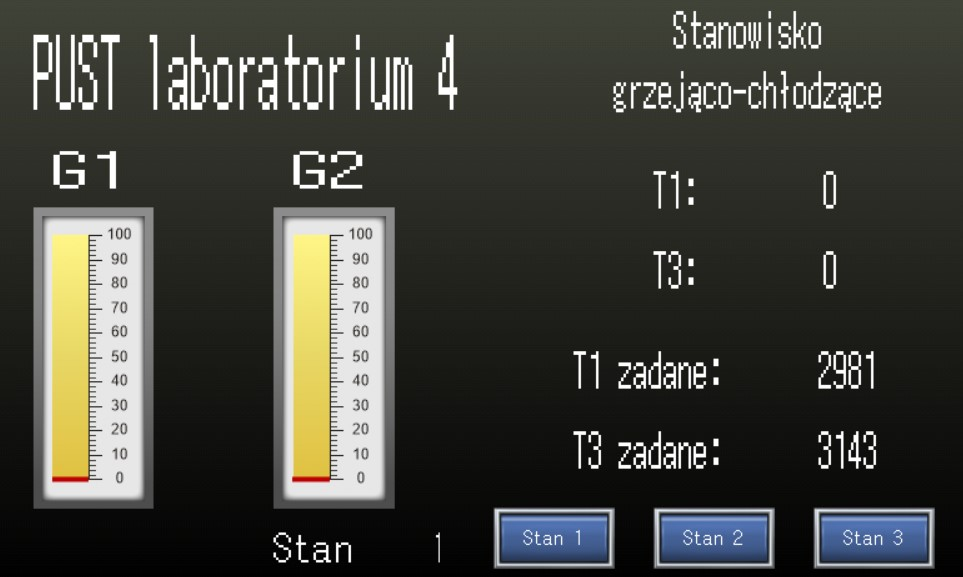
\includegraphics[width=160mm]{../images/laby/podpunkt5.jpg}
    \caption{Wygląd interfejsu użytkownika}
    \label{fig:normal}
    \end{figure}  

Na interfejsie użytkownika po prawej stronie można zauważyć słupki, które obrazują wartości grzałek G1, G2 (od 0 do 100\%). Po prawej stronie pod tytułem widnieją wartości zmierzonych temperatur (T1 oraz T3), pod nimi są wartości zadane tych wyjść. Na samym dole są 3 przyciski zmieniające stan automatu (a zboku widnieje napis mówiący, w którym stanie aktualnie się znajduje) opisanego w następnym podrozdziale.

%%%%%%%%%%%%%% Podpunkt4
\section{Automat stanów}

\begin{lstlisting}[style=customc,frame=single, caption=Implementacja automatu stanów , label=lst:overheat_lock] 
CASE Stan1 OF
	//M11 przycisk do zmiany na stan 1
	//M12 przycisk do zmiany na stan 2
	//M13 przycisk do zmiany na stan 3
	1:
	y_zad1 := 2981; //wartosci zadane dla stanu 1
	y_zad2 := 3143;
	IF M12 THEN
		Stan1 := 2;
	END_IF;
	IF M13 THEN
		Stan1 := 3;
	END_IF;
	2:
	y_zad1 := 3500; //wartosci zadane dla stanu 2
	y_zad2 := 5000;
	IF M11 THEN
		Stan1 := 1;
	END_IF;
	IF M13 THEN
		Stan1 := 3;
	END_IF;
	3:
	y_zad1 := 4000; //wartosci zadane dla stanu 3
	y_zad2 := 3500;
	IF M12 THEN
		Stan1 := 2;
	END_IF;
	IF M11 THEN
		Stan1 := 1;
	END_IF;
	
END_CASE;
\end{lstlisting} 

Zmiana stanu automatu odbywa się po wciśnięciu przycisków (widocznych na panelu operatora). Każdy z tych przycisków posiada nazwę, która informuje na jaki stan zmienia się obecny stan.
W każdym stanie zdefiniowane są inne wartości temperatór zadanych:

1. W stanie pierwszym: $T1^{zad}=29,81^{\circ} C$  $T3^{zad}=31,43^{\circ} C$

2. W stanie drugim: $T1^{zad}=35^{\circ} C$  $T3^{zad}=50^{\circ} C$

2. W stanie trzecim: $T1^{zad}=40^{\circ} C$  $T3^{zad}=35^{\circ} C$


